%%%%%%%%%%%%%%%%%%%%%%%%%%%%%%%%%%%%%%%%%%%%%%%%%%%%%%%%%%%%%%%%%%%%%%%%%%%%%%%%
%
% Template license:
% CC BY-NC-SA 3.0 (http://creativecommons.org/licenses/by-nc-sa/3.0/)
%
%%%%%%%%%%%%%%%%%%%%%%%%%%%%%%%%%%%%%%%%%%%%%%%%%%%%%%%%%%%%%%%%%%%%%%%%%%%%%%%%

%----------------------------------------------------------------------------------------
%	PACKAGES AND OTHER DOCUMENT CONFIGURATIONS
%----------------------------------------------------------------------------------------

\documentclass[
11pt, % The default document font size, options: 10pt, 11pt, 12pt
%oneside, % Two side (alternating margins) for binding by default, uncomment to switch to one side
%chapterinoneline,% Have the chapter title next to the number in one single line
spanish,
singlespacing, % Single line spacing, alternatives: onehalfspacing or doublespacing
%draft, % Uncomment to enable draft mode (no pictures, no links, overfull hboxes indicated)
%nolistspacing, % If the document is onehalfspacing or doublespacing, uncomment this to set spacing in lists to single
%liststotoc, % Uncomment to add the list of figures/tables/etc to the table of contents
%toctotoc, % Uncomment to add the main table of contents to the table of contents
parskip, % Uncomment to add space between paragraphs
%codirector, % Uncomment to add a codirector to the title page
headsepline, % Uncomment to get a line under the header
]{MastersDoctoralThesis} % The class file specifying the document structure

\usepackage[utf8]{inputenc}
\usepackage{biblatex} 
%\addbibresource{references.bib}

%----------------------------------------------------------------------------------------
%	INFORMACIÓN DE LA MEMORIA
%----------------------------------------------------------------------------------------

\thesistitle{Robot de exploración ambiental} % El títulos de la memoria, se usa en la carátula y se puede usar el cualquier lugar del documento con el comando \ttitle

% Nombre del posgrado, se usa en la carátula y se puede usar el cualquier lugar del documento con el comando \degreename
\posgrado{Carrera de Especialización en Sistemas Embebidos} 
%\posgrado{Carrera de Especialización en Internet de las Cosas} 
%\posgrado{Carrera de Especialización en Intelegencia Artificial}
%\posgrado{Maestría en Sistemas Embebidos} 
%\posgrado{Maestría en Internet de las cosas}

\author{Ing. Gonzalo Carreño} % Tu nombre, se usa en la carátula y se puede usar el cualquier lugar del documento con el comando \authorname

\director{Esp. Ing. Sergio Alberino (UTN.BA)} % El nombre del director, se usa en la carátula y se puede usar el cualquier lugar del documento con el comando \dirname
% El nombre del codirector si lo hubiera, se usa en la carátula y se puede usar el cualquier lugar del documento con el comando \codirname.  Para activar este campo se debe descomentar la opción "codirector" en el comando \documentclass, línea 23.

\juradoUNO{Nombre del jurado 1 (pertenencia)} % Nombre y pertenencia del un jurado se usa en la carátula y se puede usar el cualquier lugar del documento con el comando \jur1name
\juradoDOS{Nombre del jurado 2 (pertenencia)} % Nombre y pertenencia del un jurado se usa en la carátula y se puede usar el cualquier lugar del documento con el comando \jur2name
\juradoTRES{Nombre del jurado 3 (pertenencia)} % Nombre y pertenencia del un jurado se usa en la carátula y se puede usar el cualquier lugar del documento con el comando \jur3name

\ciudad{Ciudad Autónoma de Buenos Aires}

\fechaINICIO{marzo de 2023}
\fechaFINAL{noviembre de 2023}


\keywords{Sistemas embebidos, FIUBA} % Keywords for your thesis, print it elsewhere with \keywordnames


\begin{document}


\frontmatter % Use roman page numbering style (i, ii, iii, iv...) for the pre-content pages

\pagestyle{plain} % Default to the plain heading style until the thesis style is called for the body content



%----------------------------------------------------------------------------------------
%	RESUMEN - ABSTRACT 
%----------------------------------------------------------------------------------------

\begin{abstract}
\addchaptertocentry{\abstractname} % Add the abstract to the table of contents
%
%The Thesis Abstract is written here (and usually kept to just this page). The page is kept centered vertically so can expand into the blank space above the title too\ldots
\centering
%\usepackage{lipsum}

\graphicspath{ {./Figures/} }

\begin{center}
El presente trabajo describe un emprendimiento personal en el que se desarrolla un dispositivo robótico de exploración ambiental, controlable a distancia con las funciones básicas de desplazamiento, medición y reporte de parámetros ambientales tales como presión, temperatura, humedad y luminosidad. 
\end{center}
\begin{center}
El sistema cuenta con una arquitectura base robusta y flexible sobre la cual otros sensores y actuadores pueden ser adaptados para poder interacturar con el medio ambiente, y logra por tanto brindar una solución que ayuda a incrementar la oferta de robots exploradores en la industria argentina pudiendo ser utilizados en casos de uso de IoT, como por ejemplo en aplicaciones de explotación de petróleo, Smart Mining, Smart Farming, etc. 

\end{center}
\begin{center}
Para su implementación se utilizaron conceptos y herramientas tales como buenas prácticas en el diseño y desarrollo de firmware, la utilización de sistemas operativos de tiempo real como plataforma de ejecución base, protocolos de comunicaciones para sistemas embebidos, y técnicas y frameworks de testing para asegurar la calidad del producto final. 
\end{center}



\end{abstract}

%----------------------------------------------------------------------------------------
%	CONTENIDO DE LA MEMORIA  - AGRADECIMIENTOS
%----------------------------------------------------------------------------------------

\begin{acknowledgements}
%\addchaptertocentry{\acknowledgementname} % Descomentando esta línea se puede agregar los agradecimientos al índice
\vspace{1.5cm}

Esta sección es para agradecimientos personales y es totalmente \textbf{OPCIONAL}.  

\end{acknowledgements}

%----------------------------------------------------------------------------------------
%	LISTA DE CONTENIDOS/FIGURAS/TABLAS
%----------------------------------------------------------------------------------------

\tableofcontents % Prints the main table of contents

\listoffigures % Prints the list of figures

\listoftables % Prints the list of tables


%----------------------------------------------------------------------------------------
%	CONTENIDO DE LA MEMORIA  - DEDICATORIA
%----------------------------------------------------------------------------------------

\dedicatory{\textbf{Dedicado a mi familia y mis amigos.}}  % escribir acá si se desea una dedicatoria

%----------------------------------------------------------------------------------------
%	CONTENIDO DE LA MEMORIA  - CAPÍTULOS
%----------------------------------------------------------------------------------------

\mainmatter % Begin numeric (1,2,3...) page numbering

\pagestyle{thesis} % Return the page headers back to the "thesis" style

% Incluir los capítulos como archivos separados desde la carpeta Chapters

% Chapter 1

\chapter{Introducción general} % Main chapter title

\label{Chapter1} % For referencing the chapter elsewhere, use \ref{Chapter1} 
\label{IntroGeneral}

%----------------------------------------------------------------------------------------

% Define some commands to keep the formatting separated from the content 
\newcommand{\keyword}[1]{\textbf{#1}}
\newcommand{\tabhead}[1]{\textbf{#1}}
\newcommand{\code}[1]{\texttt{#1}}
\newcommand{\file}[1]{\texttt{\bfseries#1}}
\newcommand{\option}[1]{\texttt{\itshape#1}}
\newcommand{\grados}{$^{\circ}$}

%----------------------------------------------------------------------------------------

%\section{Introducción}
Esta sección presenta la motivación, alcance, objetivos y requerimientos del producto en el marco del estado del arte y su importancia en la industria.  

%----------------------------------------------------------------------------------------
\section{Motivación}

La motivación del presente trabajo fue primeramente volcar y unificar en un emprendimiento personal los conceptos aprendidos en la especialización de Sistemas Embebidos, con una arquitectura robusta que pueda ser extrapolada a otros casos de uso de valor en la industria como por ejemplo la exploración de suelos en el agro, la exploración submarina para la perforación de pozos de petróleo, o los mencionados más adelante en el estado del arte.
Por otra parte, se buscó desarrollar un producto que pueda contribuir a aumentar la oferta de dispositivos robóticos exploradores en Argentina.

\section{Estado del arte}

Los robots exploradores son dispositivos robotizados capaces de moverse de forma autónoma, y/o controlados a distancia, que han sido creados con el fin de reconocer y explorar un lugar o entorno donde una persona no pueda o deba acceder ya sea por motivos de capacidad, practicidad o seguridad. Por este motivo, en función de las necesidades de desplazamiento, existen diferentes sistemas de motricidad, como son por ejemplo, los bípedos, cuadrúpedos, con ruedas, tracción oruga, acuáticos/sumergibles, aéreos, etc. En cuanto a la forma de control, los hay manejados por control remoto cableado o inalámbrico, habiendo equipos más sofisticados, que gracias a aplicaciones de Inteligencia Artificial, están preparados para desplazarse y tomar decisiones de forma autónoma. Algunos de los tipos de robots exploradores más conocidos son los espaciales, de minas, de rescate en catástrofes, de tuberías, submarinos, y de suelos.

Tanto en el ámbito académico como en la industria existen trabajos, proyectos, e implementaciones comerciales similares al presente trabajo, como por ejemplo: 

\begin{itemize}
	\item El prototipo robótico de exploración minera publicado en varios artículos \cite{latam-mining-robot-minero-unsj}, \cite{diario-de-cuyo-prototipo-robotico}, e impulsado por el Instituto de Automática de la Facultad de Ingeniería de la Universidad Nacional de San Juan en el marco de un convenio con la Comisión Nacional de Energía Atómica y el Gobierno argentino \cite{comunicacion-unsj-prototipo-convenio}.

	\item El robot de exploración terrestre denominado Geobot \cite{geobot} desarrollado por los ingenieros Nelson Dario García Hurtado y Melvin Andrés González Pino, de la universidad de Pamplona, capaz de realizar reconocimiento de zonas y manipulación de muestras de manera autónoma o asistida.

	\item El robot minero MIN-SIS 1.0 SDG-STR \cite{min-sis} desarrollado por los ingenieros Hernán L. Helguero Velásquez y Rubén Medinaceli Tórrez de la Universidad Técnica de Oruro, capaz de detectar gases, almacenar datos locales y enviar video e imágenes al puesto de mando.

	\item Spot \cite{spot}, desarrollado por Boston Dynamics, un robot explorador cuadrupedo de propósito general capaz de explorar, almacenar y enviar información en tiempo real.
	  
	\item BIKE \cite{bike_inspection}, desarrollado por Waygate Technologies, un robot con ruedas magnéticas, muy utilizado en la industria de petróleo y gas entre otras, capaz de desplazarse por el interior de tuberías para poder realizar inspecciones y comunicar hallazgos.

\end{itemize}






%----------------------------------------------------------------------------------------

\section{Alcance y objetivos}
A continuación se detallan las funcionalidades incluidas en el alcance del trabajo.

\begin{itemize}
	\item Sistema de desplazamiento terrestre.
	\item Operaciones de exploración
	\begin{itemize}	
		 \item Medición de humedad ambiental.
		 \item Medición de temperatura ambiental.
		 \item Medición de presión ambiental.
		 \item Medición de luminosidad ambiental.
	\end{itemize}

	\item Visualización de estado de exploración (lecturas de los sensores).
	\item Sistema de control por medio de un joystick cableado.
\end{itemize}

Queda fuera del alcance:
\begin{itemize}
	\item Locomoción por cualquier otro medio que no sea terrestre.
	\item Cualquier otra función no contemplada en este alcance.
\end{itemize}

%----------------------------------------------------------------------------------------



\section{Requerimientos}
A continuación se listan los requerimientos del producto:
\begin{enumerate}	
	
	\item Requerimientos funcionales		
	\begin{enumerate}			
		\item El sistema debe contar con funciones de desplazamiento para poder moverse hacia adelante y atrás, y poder girar radialmente un ángulo de 360 grados.			
		\item El sistema debe ser capaz de realizar las siguientes operaciones de exploración:			
			\begin{itemize}
				\item Medición de humedad ambiental.				
				\item Medición de temperatura ambiental.				
				\item Medición de luminosidad ambiental.				
				\item Medición de presión ambiental.			
			\end{itemize}			
		\item El sistema debe poder ser controlado a distancia mediante un joystick para que el dispositivo pueda realizar sus movimientos. En caso de que alguna de sus operaciones de exploración requiera algún otro mecanismo de control, el mismo también será integrado en el joystick.		
		\item El sistema debe proveer un mecanismo de visualización de las operaciones de exploración al usuario que controla el dispositivo para poder ver el estado y lectura de las operaciones de exploración.		
		\begin{itemize}	
			\item La interfaz de usuario debe permitir visualizar las lecturas de cada uno de los sensores.
			\item Debe haber una pequeña leyenda de la magnitud que se está midiendo y la unidad utilizada junto con el valor.
		\end{itemize}		
		
	\end{enumerate}	
	
	\item Requerimientos no funcionales		
		\begin{enumerate}			
			\item La arquitectura del producto debe ser robusta y tolerante a fallas.
			\item A fin de maximizar la mantenibilidad, la arquitectura del producto debe estar modularizada para permitir que los diferentes módulos puedan ser integrados y orquestados separadamente.
			
		\end{enumerate}	
	
\end{enumerate}



\chapter{Introducción específica} % Main chapter title

\label{Chapter2}

%----------------------------------------------------------------------------------------
%	SECTION 1
%----------------------------------------------------------------------------------------
Esta sección presenta una breve introducción técnica a las herramientas hardware y software utilizadas en el trabajo.

\section{Tecnologías de hardware utilizadas}

\subsection{Espressif ESP32}


ESP32 \cite{ESP32} es una serie de microcontroladores embebidos en un chip con Wi-Fi y Bluetooth integrados, de bajo costo y consumo, desarrollado por \textit{Espressif Systems}. Emplea dos cores Xtensa® 32-bit LX6 CPU, incluye interruptores de antena, amplificador de potencia, amplificador de recepción de bajo ruido, un co-procesador ULP (Ultra Low Power), módulos de administración de energía y varios periféricos.
En la siguiente imagen (\ref{fig:esp32}) se puede apreciar la placa ESP32-WROOM-32D \cite{ESP32_wroom_32d_datasheet} utilizada para el desarrollo del presente trabajo.

\begin{center}
    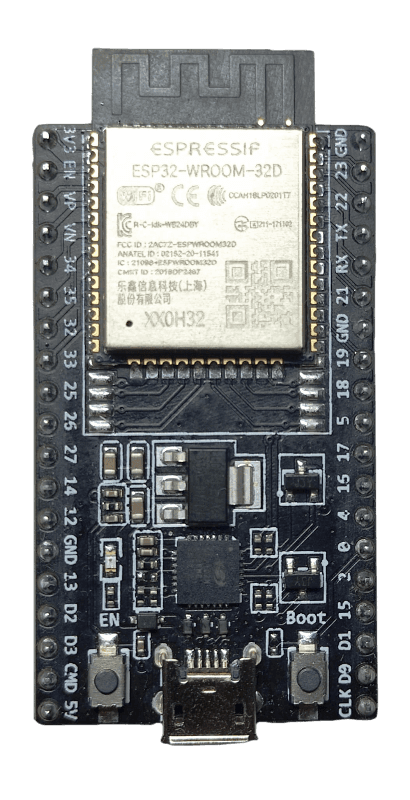
\includegraphics[scale=0.15]{electronics/esp32_2}
    \captionof{figure}{Microcontrolador ESP32-WROOM-32D.}
    \label{fig:esp32}
\end{center}


\subsection{Sensor de temperatura y humedad DHT11}

El DHT11 \cite{DHT11_datasheet} es un sensor digital de temperatura y humedad relativa de bajo costo y fácil uso. Integra un sensor capacitivo de humedad y un termistor para medir el aire circundante, y muestra los datos mediante una señal digital en el pin de datos (no posee salida analógica). Entre otras aplicaciones se lo suele utilizar principalmente en aplicaciones relacionadas al control automático de temperatura, aire acondicionado y monitoreo ambiental en agricultura. En la figura \ref{fig:dht11} se puede apreciar una imagen del componente.

\begin{center}
    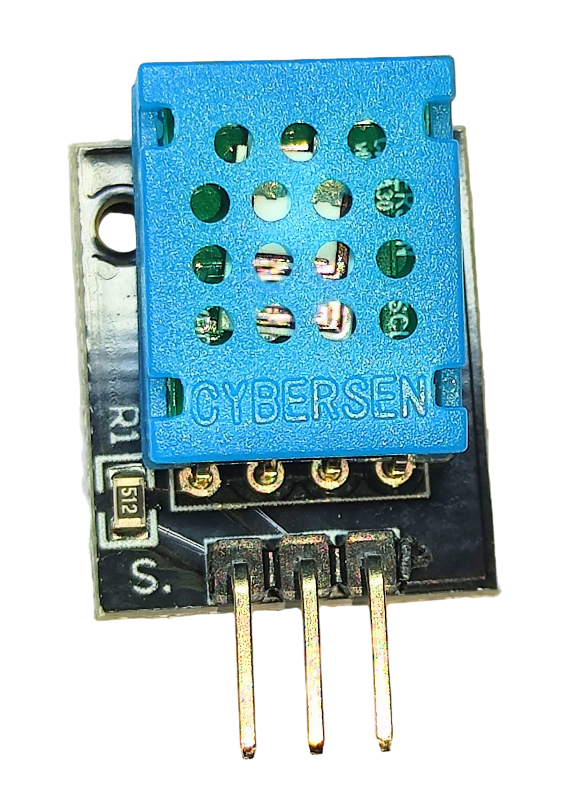
\includegraphics[scale=0.1]{electronics/dht11_2}
    \captionof{figure}{Sensor DHT11.}
    \label{fig:dht11}
\end{center}

\subsection{Sensor de presión BMP280}

El BMP280 \cite{BMP280_datasheet} es un sensor de presión barométrica absoluta, especialmente factible para aplicaciones móviles que puede ser utilizado con I2C o SPI. Permite alta precisión y linealidad, estabilidad a largo plazo, alta robustez a un muy bajo consumo. En la figura \ref{fig:bmp280} se puede apreciar una imagen del componente.

\begin{center}
    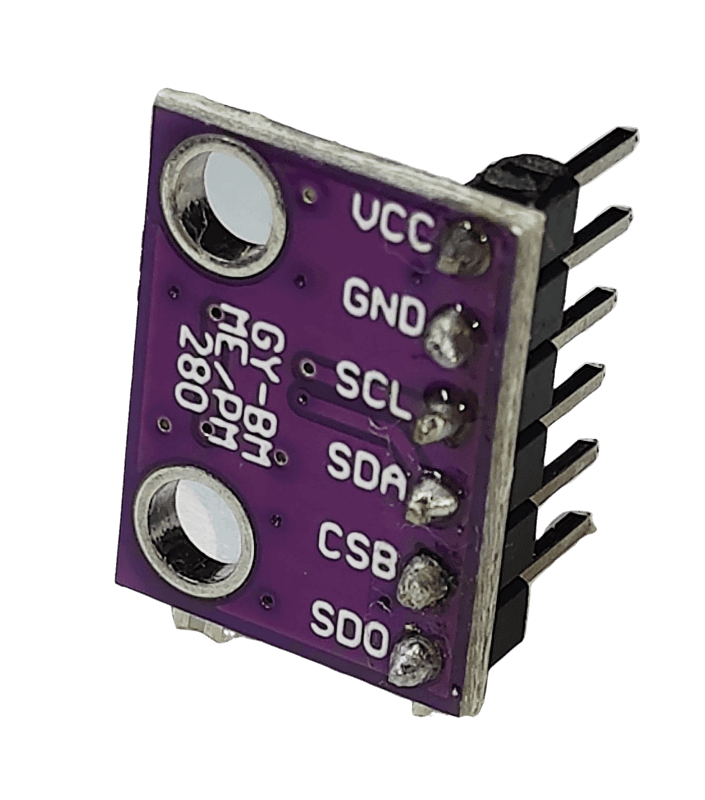
\includegraphics[scale=0.10]{electronics/bmp280_2}
    \captionof{figure}{Sensor BMP280.}
    \label{fig:bmp280}
\end{center}

\subsection{Fotoresistor como sensor de luminosidad}

El fotoresistor es una resistencia eléctrica que varía su valor en función de la cantidad de luz que incide sobre su superficie. 
Cuando el fotoresistor no está expuesto a radiaciones luminosas, los electrones están firmemente unidos en los átomos que lo conforman, por lo que alcanza su máxima resistencia eléctrica, y cuando sobre él inciden radiaciones luminosas, esta energía libera los electrones con lo cual el material se vuelve más conductor, y se disminuye su resistencia. En la figura \ref{fig:fotoresistor} se puede apreciar una imagen del componente.

\begin{center}
    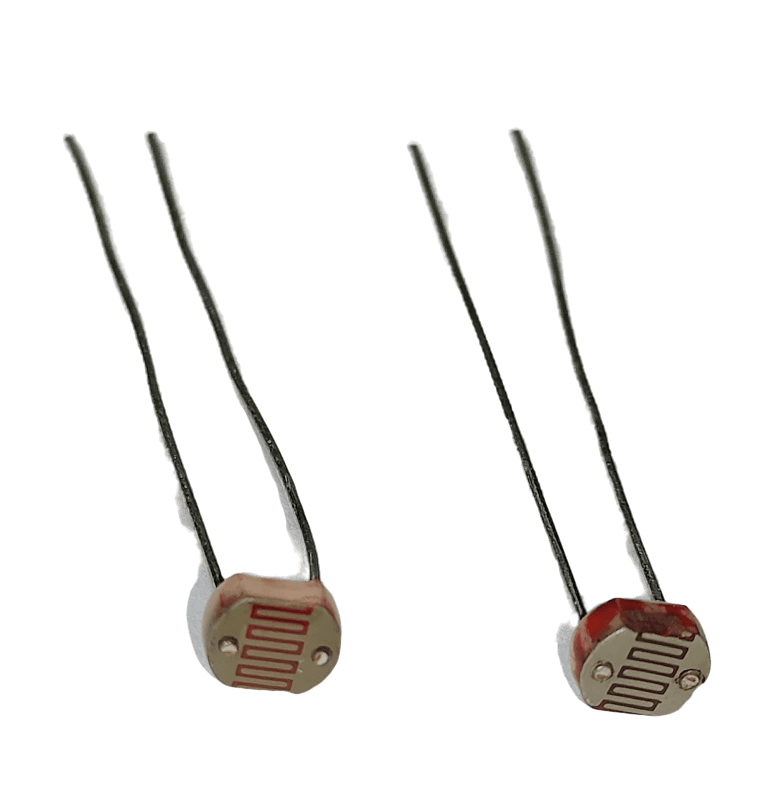
\includegraphics[scale=0.10]{electronics/fot2}
    \captionof{figure}{Fotoresistor.}
    \label{fig:fotoresistor}
\end{center}


\subsection{Joystick analógico}
 
El módulo de joystick analógico \cite{analog_joystick_datasheet} está construido sobre el montaje de dos potenciómetros en un ángulo de 90 grados. Los potenciómetros están conectados a una palanca corta centrada por resortes. 
Este módulo produce una salida de alrededor de 2,5 Volts cuando la palanca se encuentra en reposo (en el centro), mientras que al desplazarse hará que la salida varíe de 0 a 5 Volts dependiendo de su posición. La obtención de los valores en Volts se obtiene tras convertir las lecturas en niveles lógicos mediante el módulo ADC (conversor analógico digital) \cite{ESP32_adc} del microcontrolador ESP32. En la figura \ref{fig:joystick} se puede apreciar una imagen del componente.

\begin{center}
    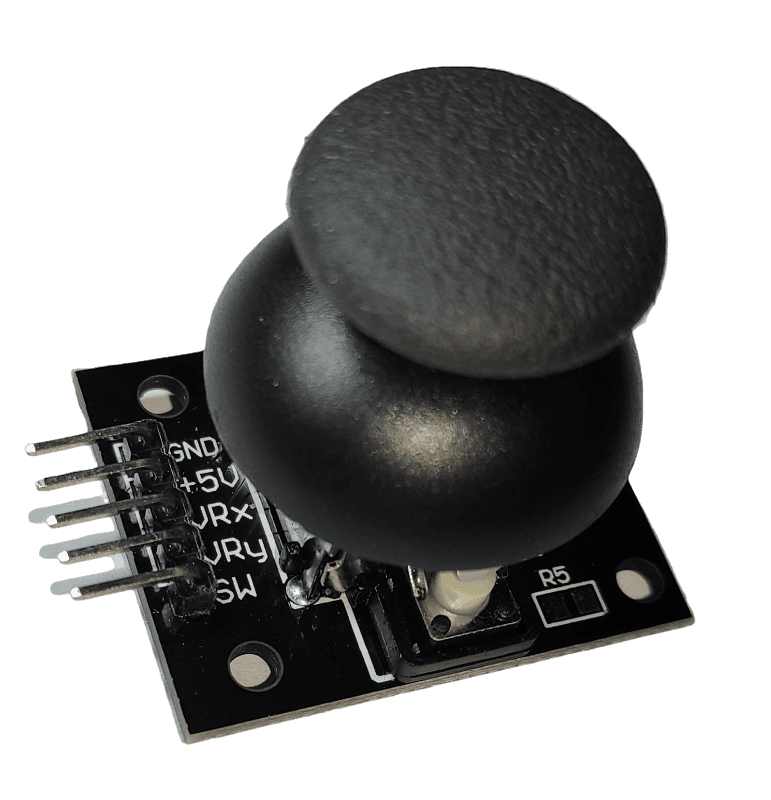
\includegraphics[scale=0.10]{electronics/joystick2}
    \captionof{figure}{Joystick analógico.}
    \label{fig:joystick}
\end{center}


\subsection{Display LCM1602A}
El display LCM1602A \cite{LCM1602A_datasheet} consta de una pantalla de cristal líquido que permite representar dos filas con hasta 16 caracteres alfanuméricos en cada una y dado que se encuentra integrada a una interfaz adaptadora I2C puede ser controlada por este protocolo. En la figura \ref{fig:display} se puede apreciar una imagen del componente.

\begin{center}
    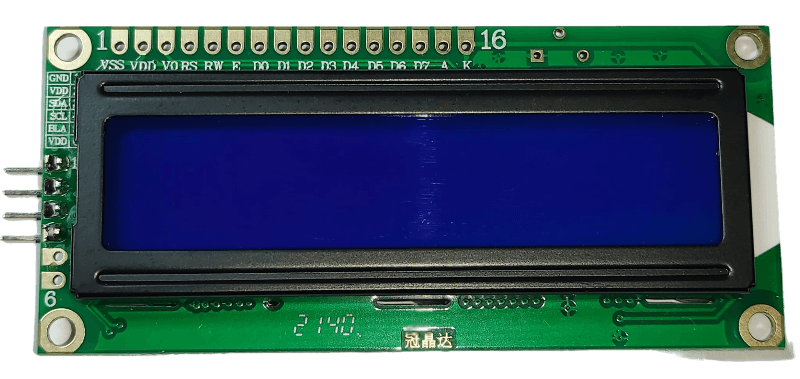
\includegraphics[scale=0.20]{electronics/display2}
    \captionof{figure}{Display LCM1602A.}
    \label{fig:display}
\end{center}

\subsection{Motores de corriente continua}
El motor DC (corriente continua) \cite{dc_motor_datasheet} es un electromotor que transforma energía eléctrica en energía mecánica. Estos motores operan con un voltaje entre 3 y 6 Volts, corriente de 150 mA, permiten una velocidad de entre 90 y 200 RPM y un torque de entre 0,15 Nm y 0,60 Nm. En la figura \ref{fig:dc_motors} se puede apreciar una imagen del componente.


%\begin{figure}[htbp]
%\centering
\begin{center}
  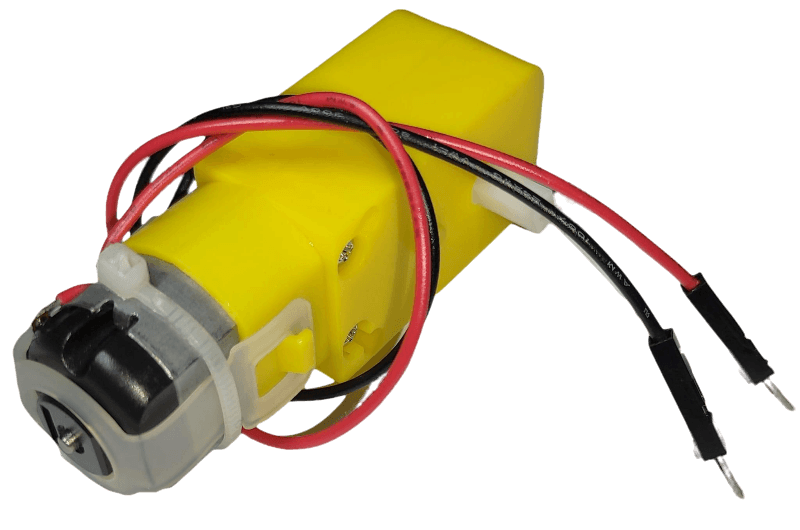
\includegraphics[scale=0.13]{electronics/engine2}
    \captionof{figure}{Motor de corriente continua.}
    \label{fig:dc_motors}
\end{center}
  
%\end{figure}


\subsection{Módulos L298N}
Los módulos L298N son controladores de motores de puente H duales muy utilizados en proyectos de robótica y automoción para controlar motores de corriente continua (DC) y motores paso a paso. El módulo se basa en el IC L298N, que es un controlador de motor de doble puente H fabricado por STMicroelectronics. Este módulo posee dos puentes H que permiten controlar 2 motores DC o un motor paso a paso bipolar/unipolar. El módulo permite controlar el sentido de giro y velocidad mediante señales TTL (transistor-transistor logic) que se pueden obtener de microcontroladores. Tiene integrado un regulador de voltaje de 5V encargado de alimentar la parte lógica del L298N cuya configuración se hace a través de un Jumper y se puede usar para alimentar el microcontrolador.

\begin{center}
   \centering
   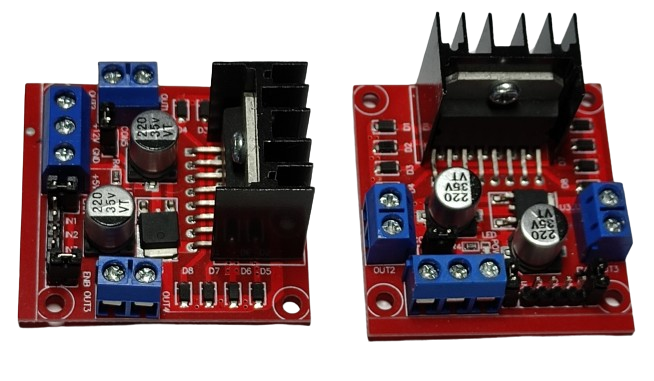
\includegraphics[scale=0.25]{electronics/l298n}
   \captionof{figure}{Interruptores de On-Off}
   \label{fig:l298n}
\end{center}

\subsection{Pilas de Li-Ion 3.7 V}
Las pilas 18650 de 3000 mAh son baterías recargables que utilizan tecnología de iones de litio y se emplean comúnmente en una variedad de dispositivos electrónicos, como por ejemplo linternas de alta potencia, laptops, vehículos eléctricos (como bicicletas y scooters), etc. Las baterías de iones de litio son conocidas por su alta densidad de energía, su baja tasa de autodescarga y su larga vida útil en comparación con otras tecnologías de baterías recargables. Con 3000 mAh (miliamperios-hora), estas baterías ofrecen una duración prolongada, lo que es ideal para dispositivos que requieren mucha energía. Al ser recargables, son más ecológicas y económicas a largo plazo en comparación con las baterías desechables. Además, son generalmente seguras y tienen una buena estabilidad térmica, reduciendo el riesgo de explosiones o incendios.

\begin{center}
   \centering
   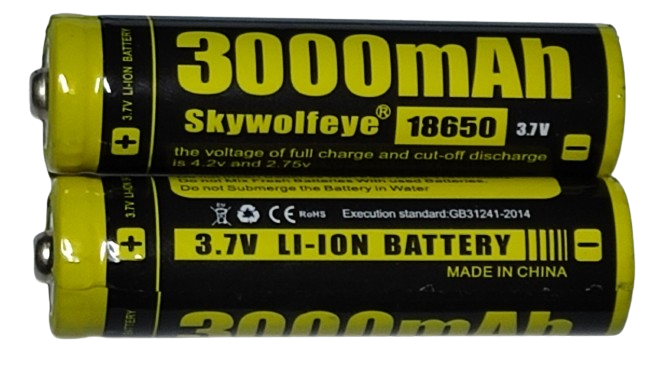
\includegraphics[scale=0.2]{electronics/baterias_liion}
   \captionof{figure}{Baterias Li-Ion}
   \label{fig:baterias_liion}
\end{center}

\subsection{Baterías AA 1.5 V}

Las pilas AA de 1.5V con 2600 mWh son baterías de tamaño AA que proporcionan una tensión de 1.5 voltios y tienen una capacidad energética de 2600 miliwatts-hora (mWh). Ofrecen alta capacidad  pudiendo durar más tiempo entre recargas o reemplazos en comparación con las baterías de menor capacidad, y versatilidad, ya que al ser AA son compatibles con la mayoría de los dispositivos electrónicos que requieren alimentación de bajo voltaje.
Las pilas AA de 1.5V con una alta capacidad como 2600 mWh son ideales para dispositivos que requieren un mayor consumo de energía, tales como cámaras digitales, linternas, juguetes electrónicos, mandos a distancia, controles de videojuegos, etc.
\begin{center}
   \centering
   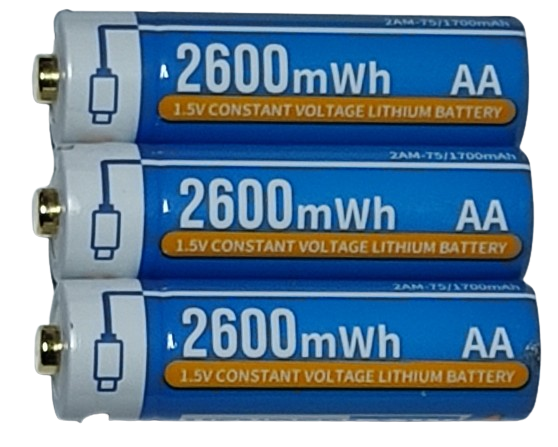
\includegraphics[scale=0.2]{electronics/pilasAA}
   \captionof{figure}{Baterías AA}
   \label{fig:pilasAA}
\end{center}


\subsection{Plaquetas genéricas PCB}
Las plaquetas electrónicas genéricas del tipo PCB (Printed Circuit Board), también conocidas como placas de desarrollo, son herramientas utilizadas principalmente en la educación, el diseño y el prototipado de circuitos electrónicos que constan de material aislante con patrones de cobre en una o ambas caras, donde se pueden soldar componentes para crear circuitos permanentes. Permiten el montaje de circuitos electrónicos de manera más duradera y fiable que el uso de un Protoboard y son asequibles de forma online a un bajo costo.

\begin{center}
   \centering
   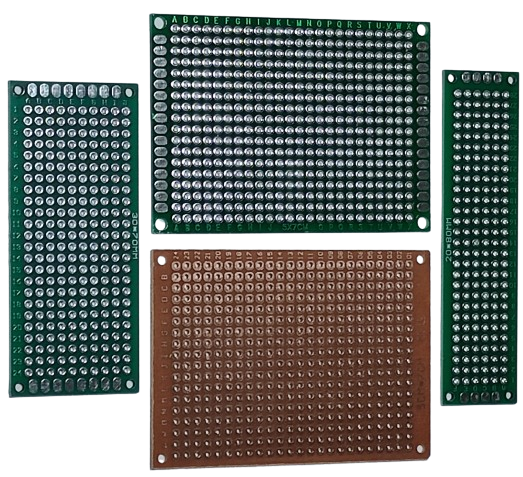
\includegraphics[scale=0.25]{electronics/plaquetas_genericas}
   \captionof{figure}{Plaquetas genericas}
   \label{fig:plaquetas_genericas}
\end{center}


\subsection{Cables de conexión DuPont}
Los cables Dupont son cables de conexión eléctrica utilizados comúnmente en prototipado y proyectos de electrónica. Estos cables son muy populares en la comunidad de los entusiastas y estudiantes de electrónica debido a su facilidad de uso y versatilidad. Están hechos de hilos de cobre con una cubierta de plástico aislante. Los conectores suelen ser de metal chapado para asegurar una buena conductividad. Los hay del tipo Hembra-Hembra, Hembra-Macho y Macho-Macho. Entre sus usos más comunes se encuentran la conexión de dispositivos en Protoboard sin necesidad de soldadura y la interconexión entre sensores, actuadores y terminales en pines o bahías de plaquetas impresas.

\begin{center}
   \centering
   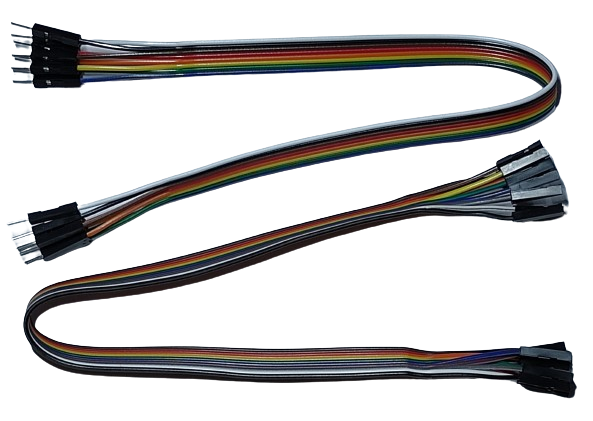
\includegraphics[scale=0.25]{electronics/dupont}
   \captionof{figure}{Cables DuPont}
   \label{fig:dupont}
\end{center}

\subsection{Board Pin Headers para montaje de componentes y cables}
Los pines de cabecera son componentes electrónicos que consisten en filas de pines metálicos montados en una base plástica. Estos pines se utilizan para realizar conexiones eléctricas entre diferentes componentes y placas en proyectos electrónicos. La cantidad de pines puede variar en número, desde unos pocos pines hasta decenas, dependiendo de las necesidades del proyecto. Pueden encontrarse en varias configuraciones, como ser Single Row -una sola fila de pines-, Double Row -dos filas de pines, aumentando la capacidad de conexión en un espacio compacto-, Right Angle -pines que se extienden en ángulo recto respecto a la base, útiles para conexiones horizontales-. Se los puede implementar con dos tipos posibles de montajes: Through-Hole (Agujero Pasante) -donde los pines se insertan a través de agujeros en la placa y se sueldan en el lado opuesto-; o bien Surface-Mount (Montaje Superficial), donde los pines se sueldan directamente en la superficie de la placa, sin pasar a través de ella.

\begin{center}
   \centering
   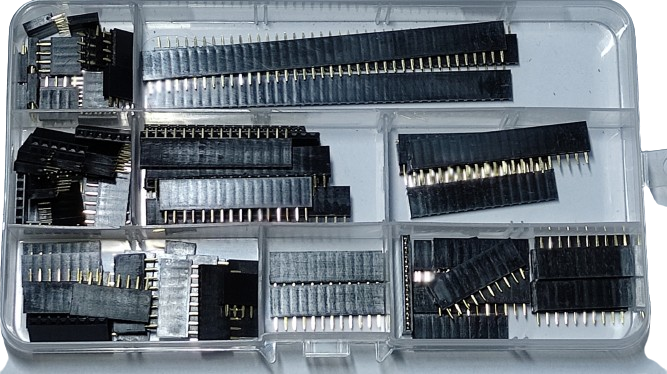
\includegraphics[scale=0.2]{electronics/pines}
   \captionof{figure}{Pines}
   \label{fig:pines}
\end{center}

\subsection{Interruptores de On-Off}
Los interruptores de encendido-apagado (on-off) son componentes fundamentales en circuitos electrónicos que permiten controlar el flujo de corriente eléctrica. Son utilizados para conectar o desconectar la corriente en un circuito, funcionando como un medio sencillo y efectivo para gestionar la energía de dispositivos electrónicos. Se los puede encontrar en diferentes tipos,     Interruptores Basculantes (Rocker Switches) -se operan basculando de una posición a otra-, interruptores deslizantes (Slide Switches) -se operan deslizando un pequeño botón a lo largo de una pista-, interruptores de palanca (Toggle Switches) -utilizan una palanca que se mueve hacia arriba y hacia abajo para cambiar entre las posiciones on y off, e interruptores de pulsador (Push-Button Switches) -al presionar el botón se conecta o desconecta el circuito-. 

\begin{center}
   \centering
   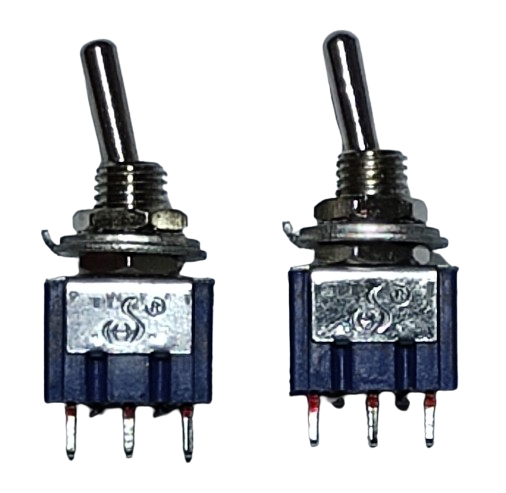
\includegraphics[scale=0.2]{electronics/interruptores}
   \captionof{figure}{Interruptores de On-Off}
   \label{fig:interruptores}
\end{center}

\subsection{Portapilas}

Los porta pilas son componentes diseñados para alojar y conectar baterías en un circuito electrónico. Estos dispositivos, generalmente hechos de plástico resistente con contactos metálicos (normalmente de níquel o acero) para asegurar una buena conductividad, facilitan la instalación y el reemplazo de baterías, asegurando una conexión segura y confiable. Se los puede encontrar comúnmente para los tipos de pilas y baterías más utilizadas, como por ejemplo AA, AAA, 9V, 18650, CR2032, etc. Además, suelen venir en tres posibles configuraciones, un solo compartimento (para una sola batería), múltiples compartimentos (para conectar varias baterías en serie o en paralelo), y con interruptor (algunos portapilas incluyen un interruptor para encender o apagar la conexión de las baterías al circuito).

\begin{center}
   \centering
   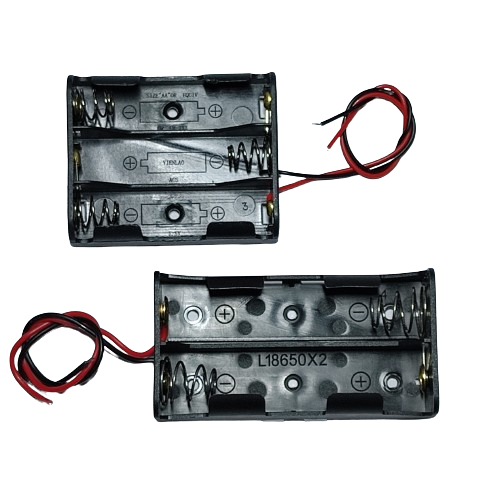
\includegraphics[scale=0.3]{electronics/porta_pilas}
   \captionof{figure}{Porta Pilas}
   \label{fig:porta_pilas}
\end{center}

\subsection{Ruedas}

Las ruedas de plástico son componentes genéricos utilizados en la comunidad hobbista y estudiantil de electrónica para el armado de sistemas con desplazamiento. Se las puede comprar online a un bajo costo, usualmente vienen en kit de dos o cuatro unidades, y son compatibles con los motores de DC utilizados para moverlas.

\begin{center}
   \centering
   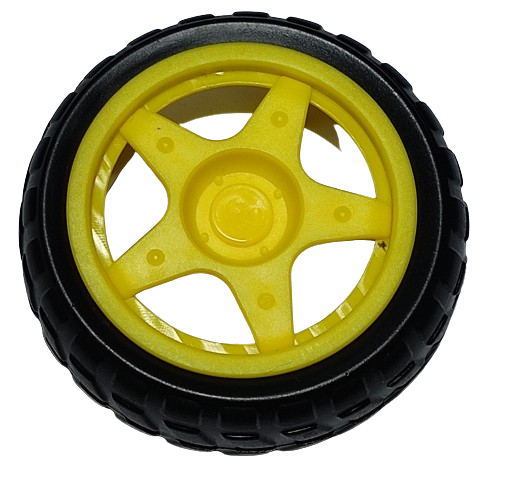
\includegraphics[scale=0.2]{electronics/ruedas}
   \captionof{figure}{Ruedas}
   \label{fig:ruedas}
\end{center}

\section{Tecnologías de software utilizadas}

\subsection{Marco de trabajo ESP-IDF}

\textit{Espressif Systems} proporciona recursos básicos de hardware y software para ayudar a los desarrolladores de aplicaciones a realizar sus ideas utilizando el hardware de la serie ESP32. El framework de software de Espressif está destinado al desarrollo de aplicaciones de IoT (Internet de las cosas) con Wi-Fi, Bluetooth, administración de energía y varias otras características del sistema.
Sus componentes son:
\begin{enumerate}
	\item Toolchain, utilizado para compilar el código para ESP32.
	\item Build tools, que provee utilidades como CMake \cite{cmake_website} y Ninja \cite{ninja_website} para construir la aplicación completa para ESP32.
	\item ESP-IDF \cite{ESPIDF_home}, que brinda la API de desarrollo para ESP32 y scripts para ejecutar Toolchain.
	
\end{enumerate}

Además de las herramientas mencionadas se utilizó el conjunto de bibliotecas y drivers provistos por el proyecto ESP-IDF-Lib \cite{esp_idf_lib_website} basados en el framework ESP-IDF.

En la figura \ref{fig:esp-idf} se puede apreciar una imagen del proceso de desarrollo y despliegue usando el framework ESP-IDF.

\begin{figure}[h]
   \centering
   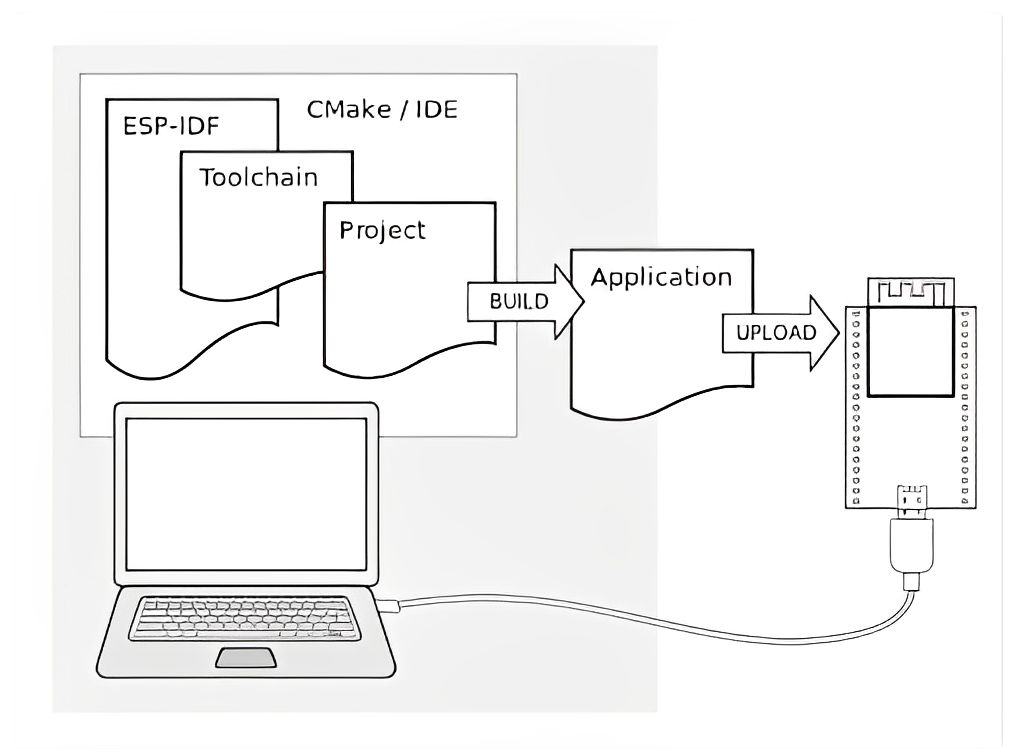
\includegraphics[scale=0.25]{conceptual/esp-idf-2}
   \caption{Proceso de desarrollo utilizando ESP-IDF\protect\footnotemark.}
   \label{fig:esp-idf}
\end{figure}

%\begin{center}
%\end{center}
%
\includegraphics[scale=0.25]{espressif}

\footnotetext{Imagen tomada de \cite{espressif-website-esp-idf}}
\subsection{Plataforma Docker}

Docker \cite{docker_website} es un proyecto de código abierto que automatiza el despliegue de aplicaciones dentro de contenedores de software, proporcionando una capa adicional de abstracción y automatización de virtualización de aplicaciones en múltiples sistemas operativos. Docker utiliza características de aislamiento de recursos del kernel Linux, tales como cgroups y espacios de nombres (namespaces) para permitir que contenedores livianos independientes se ejecuten en paralelo de manera aislada evitando la sobrecarga de iniciar y mantener máquinas virtuales.

%
\includegraphics[scale=0.15]{docker}
\subsection{Visual Studio Code}

Visual Studio Code \cite{vscode_website} es un editor de código fuente desarrollado por Microsoft para Windows, Linux, macOS y Web. Incluye soporte para la depuración, control integrado de Git, resaltado de sintaxis, finalización inteligente de código, fragmentos y refactorización de código.

%
\includegraphics[scale=0.15]{vscode}

\subsection{Sistema operativo Ubuntu}
Ubuntu \cite{ubuntu_website} es una distribución Linux basada en Debian GNU/Linux y patrocinado por Canonical, que incluye principalmente software libre y de código abierto. Puede utilizarse en ordenadores y servidores, está orientado al usuario promedio, con un fuerte enfoque en la facilidad de uso y en mejorar la experiencia del usuario.

%
\includegraphics[scale=0.25]{ubuntu}



 
\chapter{Diseño e implementación} % Main chapter title

\label{Chapter3} % Change X to a consecutive number; for referencing this chapter elsewhere, use \ref{ChapterX}

\definecolor{mygreen}{rgb}{0,0.6,0}
\definecolor{mygray}{rgb}{0.5,0.5,0.5}
\definecolor{mymauve}{rgb}{0.58,0,0.82}

%%%%%%%%%%%%%%%%%%%%%%%%%%%%%%%%%%%%%%%%%%%%%%%%%%%%%%%%%%%%%%%%%%%%%%%%%%%%%
% parámetros para configurar el formato del código en los entornos lstlisting
%%%%%%%%%%%%%%%%%%%%%%%%%%%%%%%%%%%%%%%%%%%%%%%%%%%%%%%%%%%%%%%%%%%%%%%%%%%%%
\lstset{ %
backgroundcolor=\color{white},   % choose the background color; you must add \usepackage{color} or \usepackage{xcolor}
basicstyle=\footnotesize,        % the size of the fonts that are used for the code
breakatwhitespace=false,         % sets if automatic breaks should only happen at whitespace
breaklines=true,                 % sets automatic line breaking
captionpos=b,                    % sets the caption-position to bottom
commentstyle=\color{mygreen},    % comment style
deletekeywords={...},            % if you want to delete keywords from the given language
%escapeinside={\%*}{*)},          % if you want to add LaTeX within your code
%extendedchars=true,              % lets you use non-ASCII characters; for 8-bits encodings only, does not work with UTF-8
%frame=single,	                % adds a frame around the code
keepspaces=true,                 % keeps spaces in text, useful for keeping indentation of code (possibly needs columns=flexible)
keywordstyle=\color{blue},       % keyword style
language=[ANSI]C,                % the language of the code
%otherkeywords={*,...},           % if you want to add more keywords to the set
numbers=left,                    % where to put the line-numbers; possible values are (none, left, right)
numbersep=5pt,                   % how far the line-numbers are from the code
numberstyle=\tiny\color{mygray}, % the style that is used for the line-numbers
rulecolor=\color{black},         % if not set, the frame-color may be changed on line-breaks within not-black text (e.g. comments (green here))
showspaces=false,                % show spaces everywhere adding particular underscores; it overrides 'showstringspaces'
showstringspaces=false,          % underline spaces within strings only
showtabs=false,                  % show tabs within strings adding particular underscores
stepnumber=1,                    % the step between two line-numbers. If it's 1, each line will be numbered
stringstyle=\color{mymauve},     % string literal style
tabsize=2,	                   % sets default tabsize to 2 spaces
title=\lstname,                  % show the filename of files included with \lstinputlisting; also try caption instead of title
morecomment=[s]{/*}{*/}
}


%----------------------------------------------------------------------------------------
%	SECTION 1
%----------------------------------------------------------------------------------------

Esta sección presenta los detalles técnicos del diseño e implementación de las diferentes funcionalidades del producto, la arquitectura hardware y software, y finalmente la interfaz de usuario para el control y reporte de las operaciones del robot.

El trabajo fue realizado siguiendo una metodología basada en crear un prototipo funcional con una arquitectura escalable que cumpla con alcance básico especificado en el plan de proyecto, y una vez conseguido agregar en lo posible y de acuerdo a la capacidad, funcionalidades adicionales.
De esta forma, una vez que se logró el alcance básico, considerado como la versión v1.0 del producto, se continuó con el desarrollo y se agregó la funcionalidad adicional de control inalámbrico por medio de un joystick, en lo que se considera la versión v2.0 del mismo.

En las siguientes subsecciones se detallan los detalles del diseño e implementación realizados para ambas versiones.


\section{Arquitectura de software del sistema}

Con el fin de poder lograr una arquitectura de software modular, se implementaron diferentes componentes software y servicios que abstraen el acceso a los módulos de hardware (explicados en la siguiente sección) y permite un escalamiento fácil de funcionalidades en la expansión de las funcionalidades del robot entre su versión v1.0 y la v2.0.


\subsection{Arquitectura y diseño de componentes en la versión v1.0}

A continuación se puede apreciar la arquitectura de software del sistema en su versión v1.0 y el detalle de sus componentes y servicios.

\begin{center}
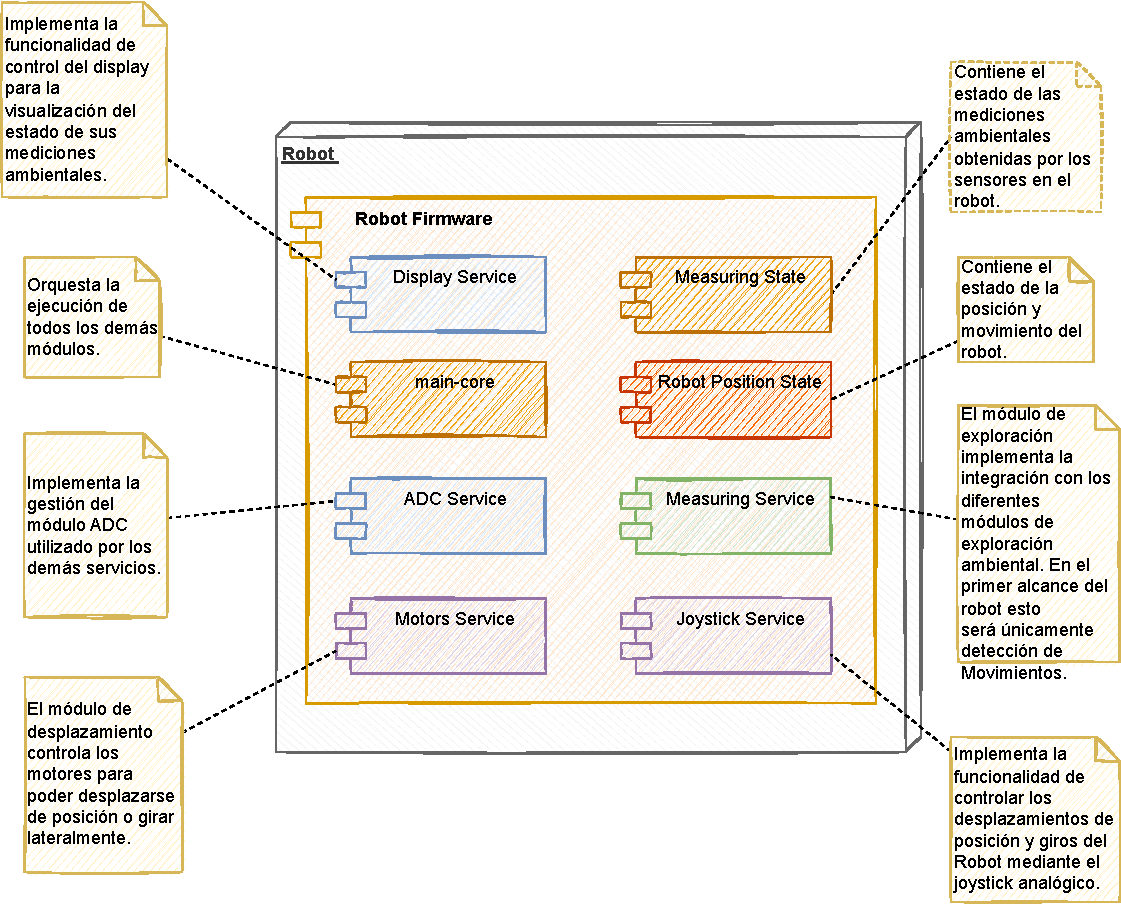
\includegraphics[scale=0.75]{software/arquitectura_software_global_v1}
  \captionof{figure}{Arquitectura global.}
  \label{fig:arquitectura_software_global}

\end{center}


Los componentes y servicios de software del Robot en la versión v1 son los siguientes:

\begin{enumerate}	
	\item Componentes de software
	\begin{enumerate}			
		\item Main-core: orquesta las diferentes tareas desde las que se invocan los demás componentes de software.
		\item Measuring Service: abstrae el acceso a los módulos de medición de temperatura, humedad, presión y luminosidad.
		\item Measuring State: mantiene el estado de cada uno de los parámetros ambientales medidos.
		\item Robot Position State: mantiene el estado del movimiento actual del robot.
		\item ADC Service: abstrae el acceso a los módulos que hacen uso de los canales que requieren conversiones ADC (analógico/digital), como el joystick analógico y el fotorresistor.
		\item Motors Service: abstrae el acceso al módulo de control de motores.
		\item Display Service: abstrae el acceso al módulo de control del display mediante I2C.
		\item Joystick Service: abstrae el acceso al módulo de control del joystick.
	\end{enumerate}	
	\item Servicios (tareas)
	\begin{enumerate}				
		\item Display Task	
		\item Measuring Task		
		\item Joystick Task
		\item Motors Task		
	\end{enumerate}			
\end{enumerate}		

\subsection{Arquitectura y diseño de componentes en la versión v2.0}

Luego de expandir su funcionalidad, los componentes y servicios de software se separaron físicamente en el hardware del robot y el del joystick, agregando además los necesarios para la comunicación inalámbrica. A continuación se puede apreciar la arquitectura de software del sistema en su versión v2.0 y el detalle de sus componentes y servicios.

\begin{center}
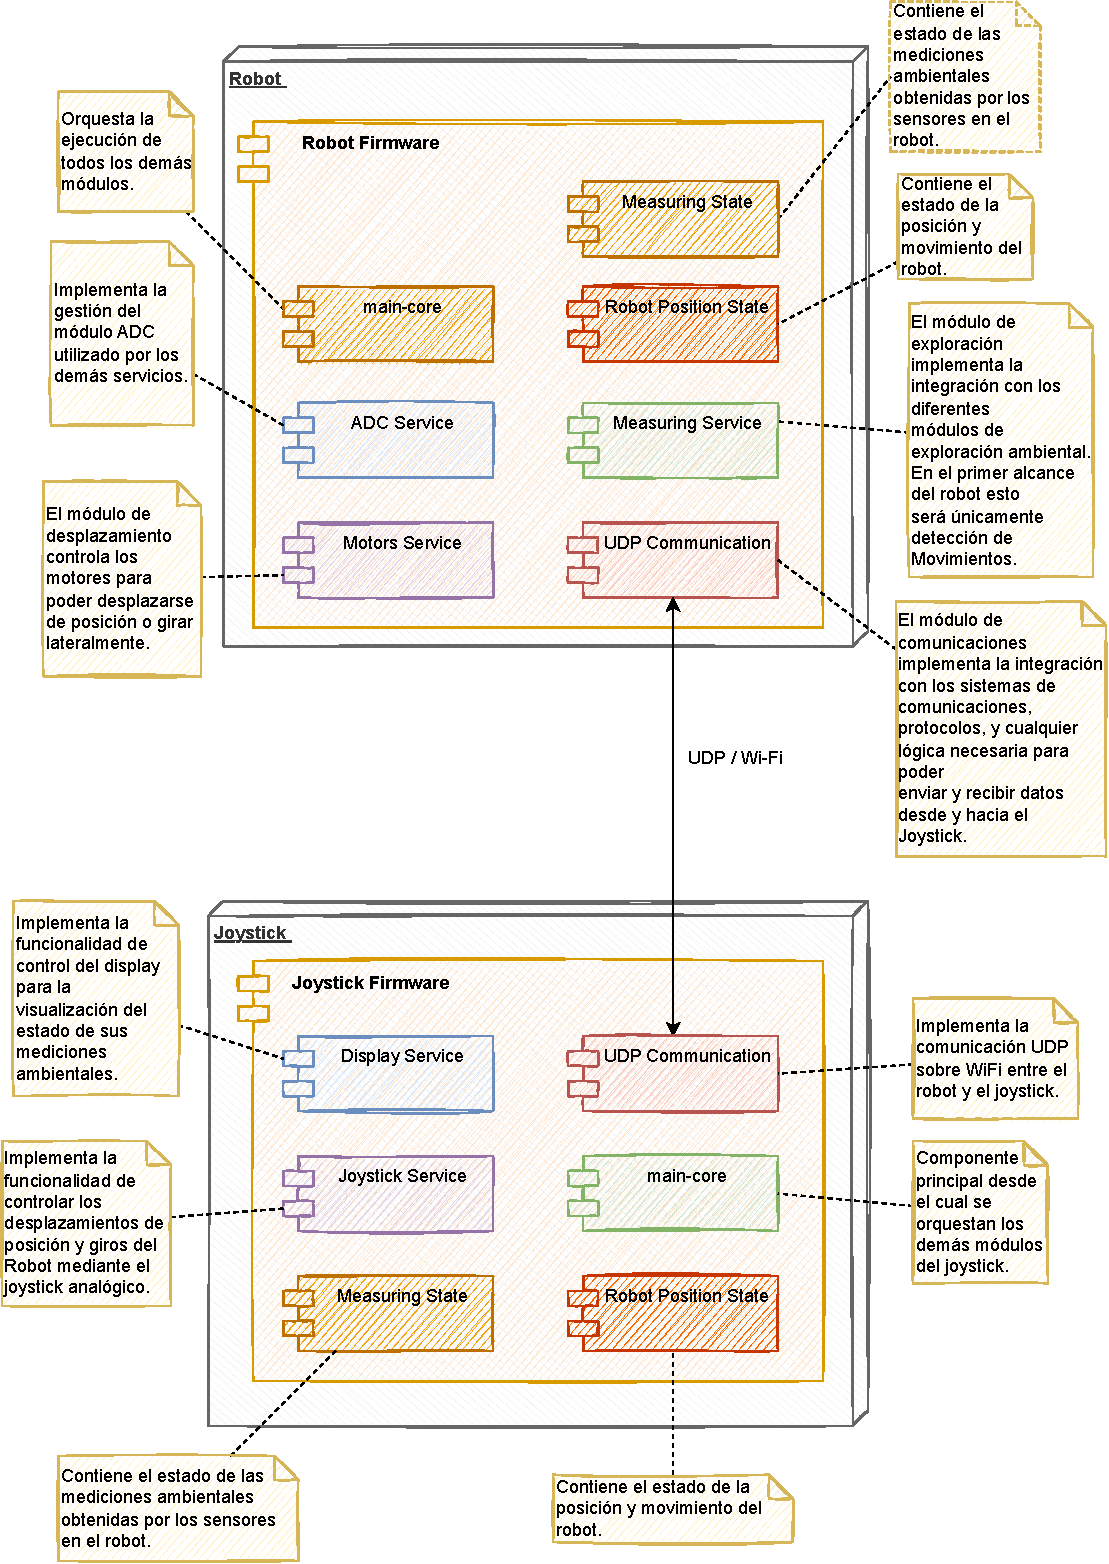
\includegraphics[scale=0.75]{software/arquitectura_software_global_v2}
  \captionof{figure}{Arquitectura global.}
  \label{fig:arquitectura_software_global}

\end{center}

Los componentes de software y servicios del robot son:

\begin{enumerate}	
	\item Componentes de software
	\begin{enumerate}			
		\item Main-core
		\item Measuring Service	
		\item Measuring State
		\item Robot Position State
		\item ADC Service
		\item Motors Service
		\item WIFI Service
		\item UDP Service	
	\end{enumerate}	
	\item Servicios (tareas)
	\begin{enumerate}				
		\item Measuring Task		
		\item Motors Task	
		\item UDP Server Task
	\end{enumerate}			
\end{enumerate}		


Los componentes de software y servicios del joystick son:

\begin{enumerate}	
	\item Componentes de software
	\begin{enumerate}			
		\item main-core
		\item Measuring State
		\item Robot Position State
		\item UDP Service	
	\end{enumerate}	
	\item Servicios (tareas)
	\begin{enumerate}				
		\item Display Task		
		\item Joystick Task	
		\item UDP Server Task
	\end{enumerate}			
\end{enumerate}		

\section{Implementación de los módulos}

Los macro componentes de hardware presentes en la arquitectura de la versión v2.0 son el robot y el joystick, que constituyen dos sistemas embebidos independientes implementados con dos microcontroladores ESP32, integrados entre sí por medio de una red WiFi y una comunicación UDP. La arquitectura de hardware del sistema esta compuesta por los siguientes módulos:


\begin{itemize}
	\item En el robot:
	\begin{itemize}
		\item Control de los motores DC.	
		\item Control de los sensores de medición (DHT11, BMP280 y fotorresistor).
		\item Gestión de la  comunicación inalámbrica vía Wi-Fi (en la versión v2.0).
	\end{itemize}
	\item En el joystick:
	\begin{itemize}
		\item Control del display.
		\item Control del joystick.
		\item Gestión de la  comunicación inalámbrica vía Wi-Fi (en la versión v2.0).
	\end{itemize}
\end{itemize}

La integración de los mismos se realizó mediante el diseño y construcción de una placa integradora central, que conecta los dispositivos hardware con el microcontrolador ESP-32.


\subsection{Control de la red Wi-Fi}

El módulo de red WiFi está integrado en el chip ESP32, el cual soporta múltiples características \cite{ESP32_WiFi} por lo tanto a nivel hardware no fue necesario realizar ningún conexionado.
A nivel de software, la gestión del módulo WiFi está incluida en el SDK ESP-IDF, y el acceso a este se realiza desde el módulo ADC 2 \cite{ESP32_adc}. Por este motivo, cuando el sistema embebido utiliza el módulo WiFi, el uso del ADC2 queda restringido a esta funcionalidad por lo tanto cualquier otro dispositivo que deba hacer uso del ADC debe ser configurado para utilizar el ADC1, como en el caso de los módulos de joystick y detección de luminosidad, que se explican en las siguientes secciones.

La configuración del \textit{soft access point Wi-Fi} implementado se realizó en base a los parámetros de red detallados en la siguiente tabla  \ref{tab:configuracion_wifi}:

\vspace{0.5cm}
\begin{table}[h]
\centering
\caption[Configuración de AP WiFi]{Configuración de AP WiFi}
\begin{tabular}{l c c}
\toprule
\textbf{Parámetro} & \textbf{Valor} \\
\midrule
SSID & Robot  \\
Password & Robot  \\
\bottomrule
\hline
\end{tabular}
\label{tab:configuracion_wifi}
\end{table}


El desarrollo de este módulo se basó en el ejemplo provisto por Espressif \cite{ESP32_WiFi_SoftAP}. El código fuente del prototipo realizado puede apreciarse en el siguiente enlace \cite{ESP32_POC_WiFi}.


\subsection{Control del joystick analógico}
Para el desarrollo de este prototipo se utilizó el SDK ESP-IDF y se configuró el módulo ADC1 de acuerdo a los siguientes detalles en la tabla \ref{fig:conexionado_joystick}:

\vspace{0.5cm}
\begin{table}[h]
\centering
\caption[Conexionado joystick]{Conexionado joystick.}
\begin{tabular}{l c c}
\toprule
\textbf{Channel} & \textbf{Unit} & \textbf{Pin GPIO}\\
\midrule
6 & 1 & 34 \\
7 & 1 & 35 \\
\bottomrule
\hline
\end{tabular}
\label{tab:conexionado_joystick}
\end{table}

A continuación, se puede apreciar el conexionado físico en la figura \ref{fig:conexionado_joystick}.

\begin{center}
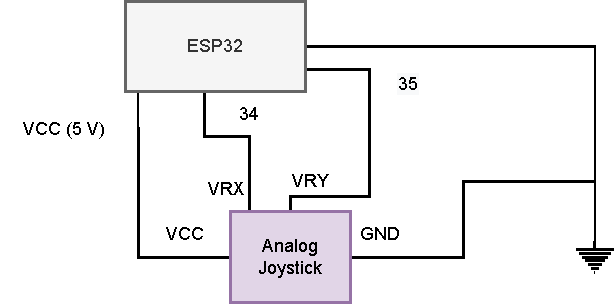
\includegraphics[scale=1]{schematics/conexionado_joystick}
  \captionof{figure}{Conexionado joystick.}
  \label{fig:conexionado_joystick}
\end{center}


El desarrollo de este módulo se basó en el ejemplo provisto por Espressif \cite{ESP32_ADC1_Example}. El código fuente del prototipo realizado puede apreciarse en el siguiente enlace \cite{ESP32_POC_joystick}.


\subsection{Medición de valor de luminosidad}
Debido a su fuerte dependencia con la temperatura, y especialmente a que su distribución espectral no resulta adecuada para la medición de iluminancia, los fotoresistores no pueden proporcionar una medición precisa de iluminancia como lo haría un luxómetro. No obstante, el fotorresistor resulta puede ser utilizado como sensor para proporcionar medidas cuantitativas sobre el nivel de luz, tanto en interiores como en exteriores.
Para leer los valores del fotorresistor se utilizó la función \textbf{adc1\textunderscore get\textunderscore raw } del SDK ESP-IDF, donde el valor devuelto se encuentra en el rango [0 - 2050], con \textit{\textbf{0}} el valor de mayor iluminación y \textit{\textbf{2050}} el menor.
Finalmente, para calcular el nivel de iluminación como valor porcentual, en el rango [0-100], siendo cero el nivel más oscuro y cien más iluminado, se utilizó la siguiente función matemática:

\begin{equation*}
\mbox{Nivel de Iluminación}=\frac{\mbox{MaxReading - reading}}{\mbox{MaxReading}} x 100
\end{equation*}

Donde:
\begin{itemize}
	\item El valor \textit{reading} es la lectura analógica del valor del fotorresistor.
	\item El valor \textit{MaxReading} es el máximo valor analógico posible de ser entregado por el fotorresistor, en este caso 2050.
	\item El valor \textit{MaxReading} es el máximo valor analógico posible de ser entregado por el fotorresistor, en este caso 0.
\end{itemize}

Para el desarrollo de este prototipo se utilizó el SDK de ESP-IDF y se configuró el módulo ADC1 de acuerdo a los detalles provistos en la tabla \ref{tab:conexionado_fotoresistor}.

\vspace{0.5cm}
\begin{table}[h]
\centering
\caption[Conexionado fotoresistor]{Conexionado fotorresistor.}
\begin{tabular}{l c c}
\toprule
\textbf{Channel} & \textbf{Unit} & \textbf{Pin GPIO}\\
\midrule
0 & 1 & 36 \\
\bottomrule
\hline
\end{tabular}
\label{tab:conexionado_fotoresistor}
\end{table}

A continuación, se puede apreciar un diagrama de su conexionado físico en la figura \ref{fig:conexionado_fotoresistor}.

\begin{center}
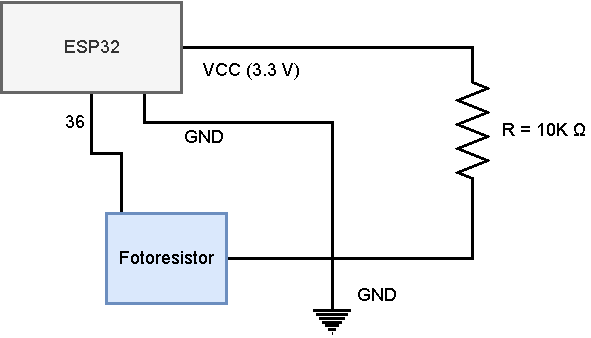
\includegraphics[scale=1]{schematics/conexionado_fotoresistor}
  \captionof{figure}{Conexionado fotorresistor.}
  \label{fig:conexionado_fotoresistor}
\end{center}

El desarrollo de este módulo se basó en el ejemplo provisto por Espressif \cite{ESP32_ADC1_Example}. El código fuente del prototipo realizado puede apreciarse en el siguiente enlace \cite{ESP32_POC_photoresistor}.

\subsection{Medición de temperatura y humedad}

Para el desarrollo de este modulo se utilizó la biblioteca de código ESP-IDF-Lib Components Library \cite{esp_idf_lib_website} que provee el soporte para gestionar el DHT11. Para acceder a las lecturas del dispositivo se abstrajo mediante el componente Measuring Service, este es invocado por la tarea Measuring Task y el estado de la lectura es almacenado en el componente Measuring State.
A continuación, se puede apreciar el conexionado del prototipo en la figura \ref{fig:conexionado_dht11}.

\begin{center}
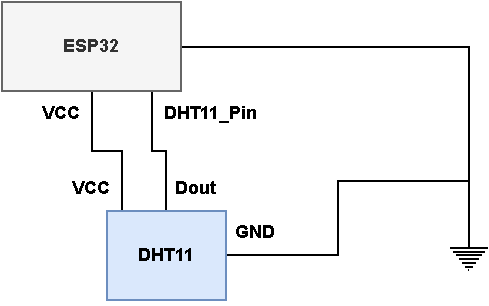
\includegraphics[scale=1]{schematics/conexionado_dht11}
  \captionof{figure}{Circuito del conexionado DHT11.}
  \label{fig:conexionado_dht11}
\end{center}

El desarrollo de este módulo se basó en el ejemplo provisto por la biblioteca ESP-IDF-Lib \cite{ESP32_dht11_example}. El código fuente del prototipo realizado puede apreciarse en el siguiente enlace \cite{ESP32_POC_dht11}.

\subsection{Medición de presión}
Para el desarrollo de este módulo se utilizó el framework ESP-IDF y la biblioteca de código ESP-IDF Components que provee el soporte para gestionar el dispositivo BMP280 por medio del protocolo I2C. El driver es inicializado en el componente main-core para ser posteriormente invocado desde el Measuring Service en la tarea Measuring Task. Sus lecturas son guardadas en el Measuring State. A continuación, se puede apreciar el conexionado del prototipo en la figura \ref{fig:conexionado_bmp280}.
\begin{center}
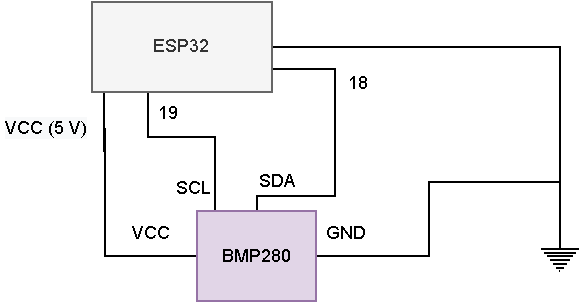
\includegraphics[scale=1]{schematics/conexionado_bmp280}
  \captionof{figure}{Conexionado BMP280.}
  \label{fig:conexionado_bmp280}
\end{center}

El desarrollo de este módulo se basó en el ejemplo provisto por la biblioteca ESP-IDF-Lib \cite{ESP32_bmp280_example}. El código fuente del prototipo realizado puede apreciarse en el siguiente enlace \cite{ESP32_POC_bmp280}.


\subsection{Control de motores DC}

Para la implementación del módulo de control de los motores de corriente continua se utilizaron a nivel de hardware dos módulos puentes L298N \cite{L298N}, que permiten integrar y controlar dos motores cada uno. Con el fin de alimentar los módulos con una fuente de poder de corriente y tensión consistente, se utilizaron dos baterías de Li-Ion de 3,7 V y 2000 mA/h conectadas en serie, activadas mediante un interruptor.
A nivel driver en el ESP32 se utilizó el módulo de control de motores por modulación de pulsos (MCPWM) \cite{ESP32_MCPWM} que por medio de la configuración de sus unidades y del \textit{duty cycle} \cite{ESP32_MCPWM_2} se puede controlar el sentido y velocidad de rotación de los motores.
Los puentes L298N proporcionan también además una tensión de salida de 5 V, y que se utilizó para la alimentación del ESP32 conectando su pin Vin.

En el siguiente diagrama puede apreciarse el conexionado lógico para el control de los motores con los componentes mencionados.

\begin{center}
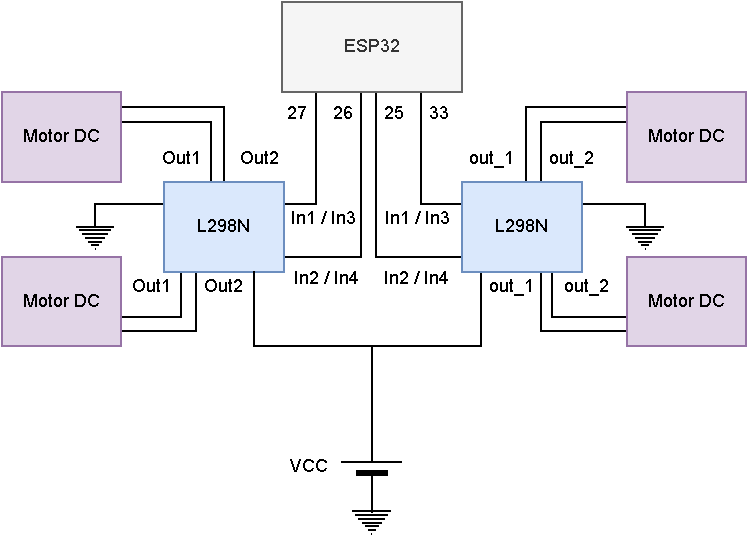
\includegraphics[scale=1]{schematics/conexionado_motores}
  \captionof{figure}{Conexionado motores.}
  \label{fig:conexionado_motores}
\end{center}

El desarrollo de este módulo se basó en el ejemplo provisto por Espressif \cite{ESP32_MCPWM_example}. El código fuente del prototipo realizado puede apreciarse en el siguiente enlace \cite{ESP32_POC_motor_MCPWM}.



\subsection{Control del display}

Para la implementación del módulo de visualización de valores observados se integró un display de dos líneas y dieciséis caracteres LCM1602A por medio de un driver I2C que facilita su control. Al basarse en el protocolo I2C el display comparte las mismas líneas SCL y SDA que el sensor BMP280.

\begin{center}
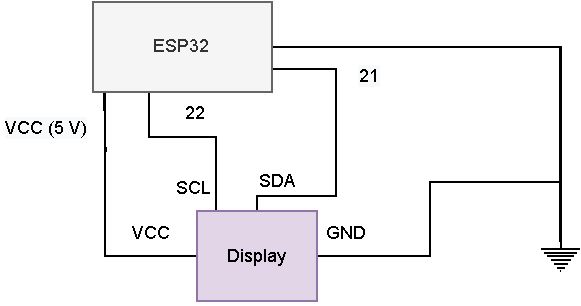
\includegraphics[scale=1]{schematics/conexionado_display}
  \captionof{figure}{Conexionado display.}
  \label{fig:conexionado_display}

\end{center}


El desarrollo de este módulo se basó en el ejemplo provisto en el enlace \cite{ESP32_Display_Example}. El código fuente del prototipo realizado puede apreciarse en el siguiente enlace \cite{ESP32_POC_display}.


\section{Arquitectura de hardware}


\subsection{Ensamblado final del producto v2.0}

En las siguientes imagenes se pueden apreciar las diferentes perspectivas del robot y del joystick.

\begin{center}
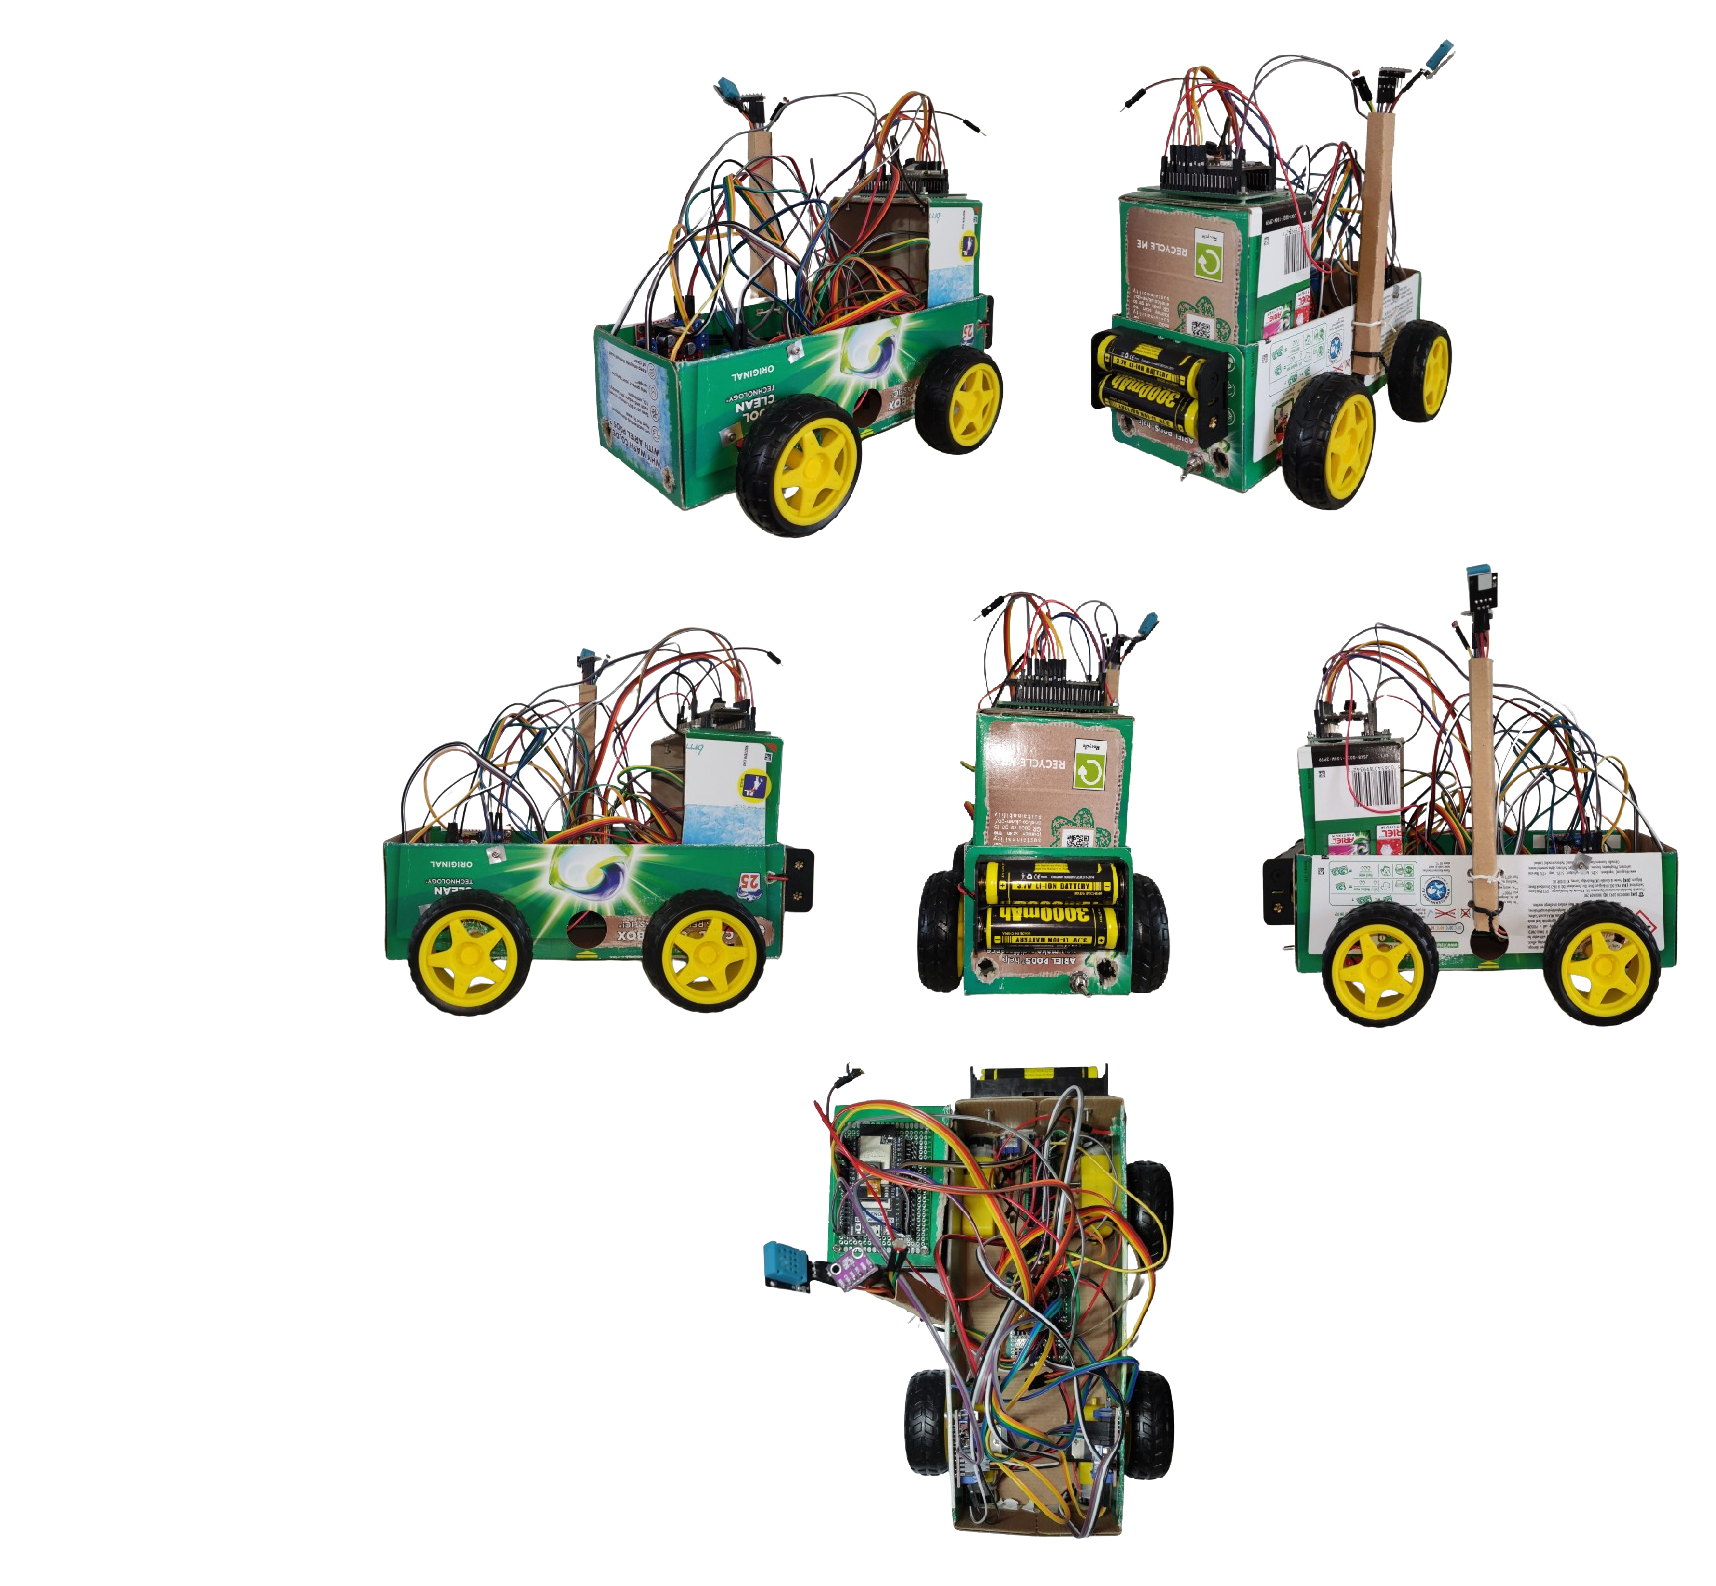
\includegraphics[scale=0.5]{demo_product/all_perspectives_robot}
  \captionof{figure}{Hardware del robot.}
  \label{fig:conexionado_fisico}
\end{center}


\begin{center}
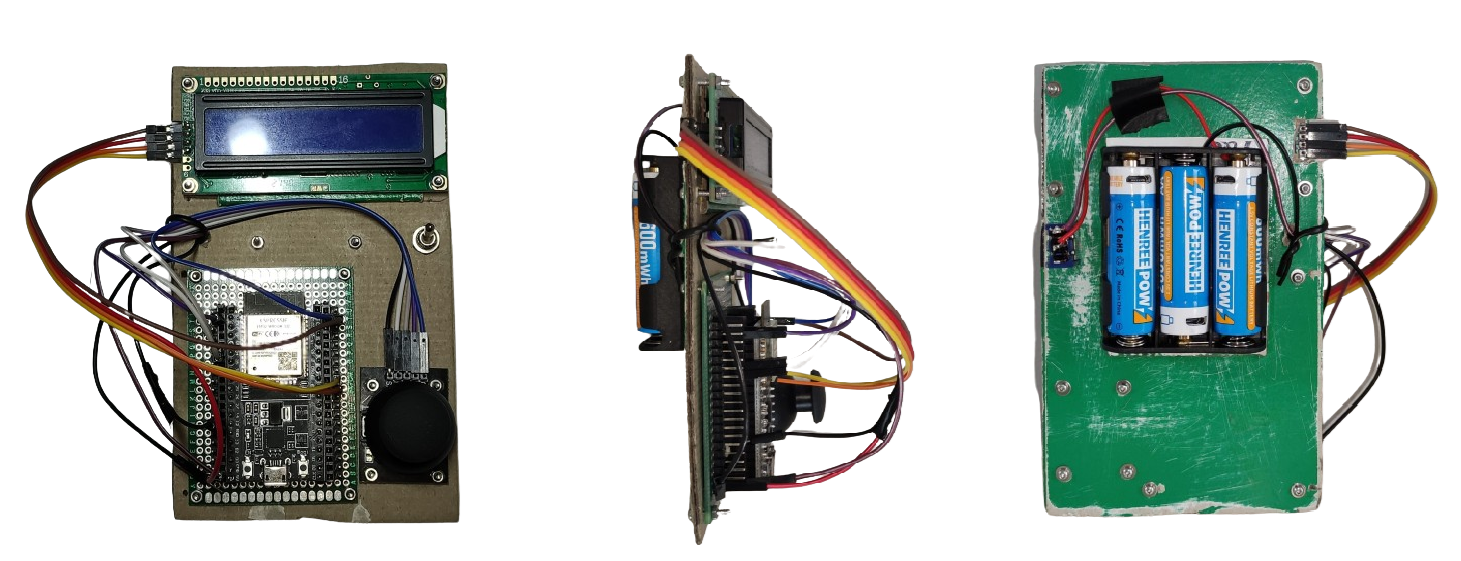
\includegraphics[scale=0.55]{demo_product/all_perspectives_joystick}
  \captionof{figure}{Hardware del joystick.}
  \label{fig:conexionado_fisico}
\end{center}



\subsection{Conexionado lógico }

En las siguientes imagenes se pueden apreciar los conexionados lógicos del robot y del joystick.

\begin{center}
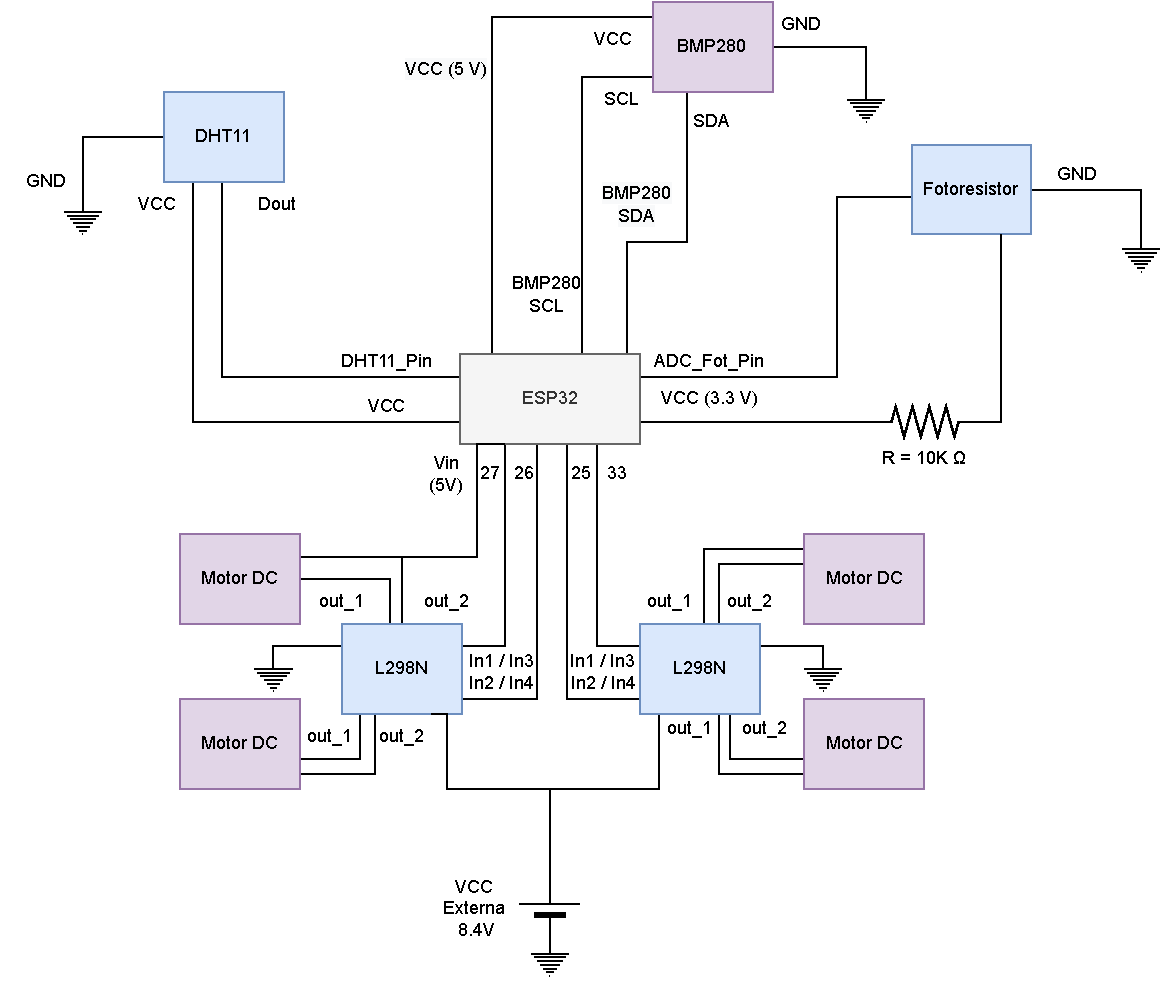
\includegraphics[scale=0.75]{schematics/conexionado_completo_robot}
  \captionof{figure}{Conexionado del robot.}
  \label{fig:conexionado_completo_robot}
\end{center}


\begin{center}
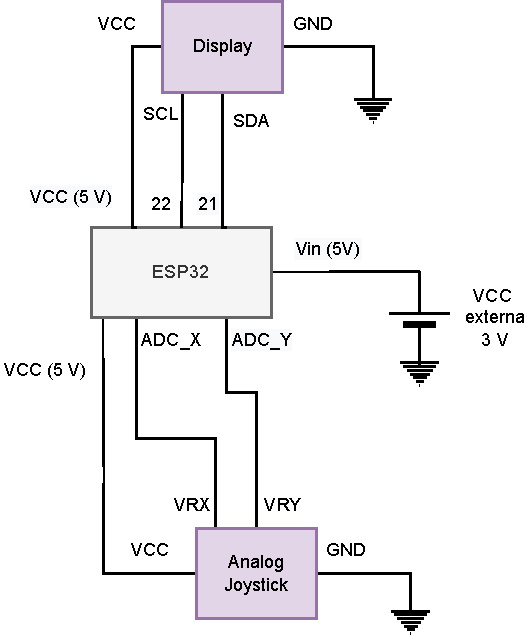
\includegraphics[scale=0.75]{schematics/conexionado_completo_joystick}
  \captionof{figure}{Conexionado del joystick.}
  \label{fig:conexionado_completo_joystick}
\end{center}


\subsection{Conexionado físico}

En la siguiente imagen se puede apreciar el conexionado fisico del robot.

\begin{center}
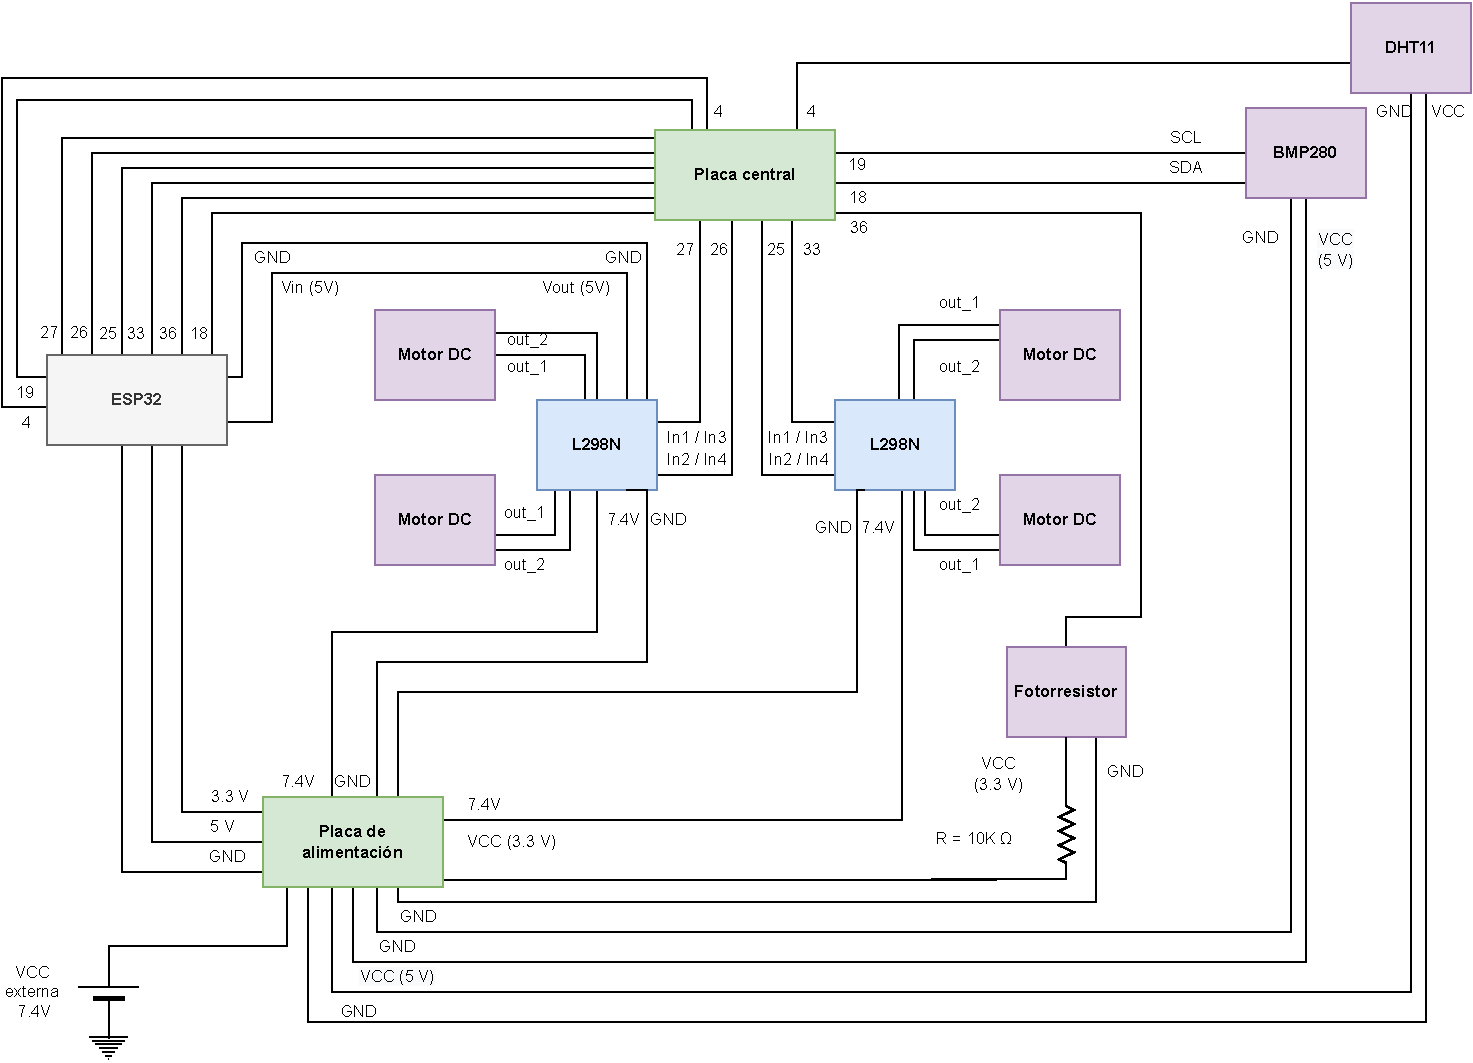
\includegraphics[scale=0.6]{schematics/conexionado_fisico}
  \captionof{figure}{Conexionado físico del robot.}
  \label{fig:conexionado_fisico}
\end{center}




\section{Ciclo de desarrollo}

Durante el ciclo de desarrollo se utilizaron las herramientas explicadas en el capítulo anterior, y se creó por cada prototipo una imagen Docker extendiendo la de espressif/idf \cite{Espressif_docker_image}. El proceso de compilación y despliegue está explicado en la documentación técnica del producto \cite{Robot_Tecnical_doc}.











% Chapter Template

\chapter{Ensayos y resultados} % Main chapter title

\label{Chapter4} % Change X to a consecutive number; for referencing this chapter elsewhere, use \ref{ChapterX}

%----------------------------------------------------------------------------------------
%	SECTION 1
%----------------------------------------------------------------------------------------
Esta sección presenta los diferentes prototipos realizados para determinar la viabilidad de cada una de las funcionalidades provistas, la metodología de desarrollo, testing, y finalmente los entregables finales del trabajo.

\section{Proceso de desarrollo y aseguramiento de calidad}
\label{sec:pruebasHW}

Para el proceso de desarrollo se realizaron pruebas de concepto de las diferentes funcionalidades utilizando como materiales la bibligrafia encontrada en internet, las hojas de datos y los ejemplos de codigo provistos por el SDK y librerias empleadas. Una vez logrado el objetivo funcional de componente se optimizo y encapsulo cada modulo para ser integrado de manera individual a un prototipo integrador sin afectar el funcionamiento de cualquier otro modulo.
De esta manera se desarrollo un prototipo integrador como la sumatoria de todos los modulos de forma incremental, probandose por regresion que los modulos ya integrados previamente siquieran funcionando de forma optima.

Una vez logrado el prototipo integrador con todas las funcionalides de la version v1.0 se prosiguio a la expansion en hardware del mismo para crear la version v2.0 extrayendo los modulos de joystick y display -que serian posteriormente agregados al sistema embebido del joystick- e incorporando los modulos de conectividad UDP sobre WiFi.

Tras lograr la version v2.0 se repitio el proceso de control de calidad de los diferentes modulos ya integrados.

A continuacion se detallan las diferentes pruebas realizadas 

\section{Verificacion tecnica de los diferentes modulos}


Todos los modulos fueron probados mediante una inspeccion visual durante el proceso de pruebas de concepto. 


\subsection{Verificacion del modulo de joystick}
Se verifico visualmente que los valores del joystick analogico puedan ser leidos apropiadamente, y que sean representativos y relevantes con la direccion del movimiento de la palanca sobre sus coordenadas X e Y.

\subsection{Verificacion del modulo de control del display}
Se verifico visualmente que el display represente los caracteres programados en la prueba de concepto con una intensidad de luz aceptable para poder leerlos apropiadamente.


\subsection{Verificacion del modulo de control de motores}
Se verifico visualmente que individualmente el motor pudiera girar en ambos sentidos. Luego, al implementarse los cuatro motores con sus ruedas, se probo que se pueda realizar los giros en todas las direcciones.

\subsection{Verificacion del modulo de medicion de temperatura y humedad}
Se verifico visualmente que los valores obtenidos por el sensor DHT11 fueran cercanos a lo esperado en relacion a la temperatura en el interior del lugar de experimentacion y la humedad en un valor cercano a lo reportado en Google.

\subsection{Verificacion del modulo de medicion de presion atmosferica}
Se verifico visualmente que el valor obtenido por el sensor BMP280 fuera cercano a lo esperado en relacion al valor reportado por Google.


\subsection{Verificacion del modulo de medicion de luminosidad}
Se verifico visualmente que los valores obtenidos del fotorresistor, tras ser transformados a valores absolutos porcentuales, guarden relacion con el nivel de luminosidad ambiental del interior de lugar de experimentacion.


\subsection{Verificacion del modulo de comunicacion UTP sobre WiFi}
Por medio de un dos programas UDP, uno cliente y uno servidor, se probo el establecimiento de la comunicacion UDP entre dos ESP32. Luego se incorporo el servicio de comunicaciones UDP en el robot y mientras que desde el programa cliente se enviaban las acciones representando las direcciones del movimiento a realizar (FORWARD, BACKWARD, LEFT, RIGHT) y se observo visualmente como el robot giraba sus ruedas en funcion de los comandos enviados. Finalmente se incorporo el modulo de comunicaciones en el joystick para enviar los comandos al robot cuando se realizaba dicho 


\section{Pruebas funcionales del producto}


\subsection{Prueba del modulo de medición de temperatura y humedad}

Se compararon los valores medidos por el modulo de medicion de temperatura y humedad basado en el sendor DHT11 con los obtenidos a traves de un dispositivo de medicion de temperatura y humedad. Se realizo la medicion en diferentes contextos:

\begin{itemize}
	\item En el interior de una vivienda.
	\item En el exterior un dia calido.
	\item En el exterior un dia frio.
\end{itemize}


\subsection{Prueba del modulo de medición de presión}

Se compararon los valores medidos por el modulo de medicion de presion basado en el sendor BMP280 con los obtenidos a traves de un dispositivo de medicion de temperatura y humedad. Se realizo la medicion en un solo lugar con la misma altitud a nivel del mar.

\subsection{Prueba del modulo de medición de luminosidad ambiental}

Se compararon los valores medidos por el modulo de medicion de luminosidad basado en un fotoresistor percibidos por el ojo humano sin utilizar ningun dispositivo de medicion. Se realizo la medicion en diferentes escenarios

\begin{itemize}
	\item En interiores con luz concentrada sobre el sensor.
	\item En interiores con luz ambiental no concentrada.
	\item En interiores con a oscuras
	\item En el exterior un dia calido.
	\item En el exterior un dia frio.
\end{itemize}

Los resultados mostraron que los valores porcentuales indicados por el modulo de medicion de luminosidad son consistentes con los niveles de luz detectados por el ojo humano.

\subsection{Prueba del control y desplazamiento del robot}

Se verifico el control y desplazamiento del robot de forma visual por medio de accionar el joystick en las diferentes coordenadas (X;Y) y controlar que la direccion del movimiento del robot sea acorde a las mismas.


\subsection{Prueba del modulo de visualización de display}

Se verifico el funcionamiento del display visualizando las lecturas de los valores sensados y transmitidos por el robot. Se verifico que 

\begin{itemize}
	\item las lecturas sean nitidas y entendibles
	\item las unidades de medida esten presentes
	\item haya un detalle de lo que se esta midiendo acompaniando las lecturas y la unidad de medida
	\item el nivel de luminosidad sea optimo para permitir la lectura independientemente de la iluminacion ambiental
	\item se presenten las lecturas de todos los valores observados 
\end{itemize}

\section{Reportes de testing}

...


\section{Documentacion del producto }

Se desarrollo la documentacion del producto compuesta de los siguientes entregables
\begin{itemize}
	\item Documentacion tecnica \cite{Robot_Tecnical_doc}.
	\item Manual de usuario \cite{Robot_User_manual}.
\end{itemize}




 
% Chapter Template

\chapter{Conclusiones} % Main chapter title

\label{Chapter5} % Change X to a consecutive number; for referencing this chapter elsewhere, use \ref{ChapterX}


%----------------------------------------------------------------------------------------

%----------------------------------------------------------------------------------------
%	SECTION 1
%----------------------------------------------------------------------------------------

% \begin{itemize}\item ¿Cuál es el grado de cumplimiento de los requerimientos?
En el presente trabajo se ha implementado un robot de exploración ambiental que cumple con todos los requerimientos establecidos en el plan de proyecto. Los requerimientos funcionales han sido abordados mediante la implementación de los módulos de desplazamiento, control de movimiento, medición de parámetros ambientales y visualización, explicados en las secciones 3 y 4. Los requerimientos de documentación han sido cubiertos con los respectivos documentos referenciados en la sección 4. Los requerimientos de testing se cumplieron a través de tests unitarios midiendo el nivel de cobertura, además de la verificación y validación funcional de cada módulo (\textit{smoke test}) explicada en la sección 4. Los requerimientos de interfaz han sido completados como parte de la implementación del módulo de visualización explicados en la sección 3 y evidenciados en la sección 4.
Finalmente, de los requerimientos opcionales se implementó la comunicación inalámbrica entre el joystick y el robot mediante UDP sobre TCP/IP.

% \item ¿Cuán fielmente se puedo seguir la planificación original (cronograma incluido)?
Con respecto a la planificación original \cite{Robot_Planificacion}, durante la implementación del trabajo se produjeron eventos que afectaron los supuestos sobre la capacidad del alumno, lo que generó el riesgo de demora en la entrega. Este riesgo, contemplado en el plan del proyecto, fue aceptado (no mitigado) para no sacrificar ni el alcance ni la calidad, lo que resultó en un retraso en el plan original.


% \item ¿Se manifestó algunos de los riesgos identificados en la planificación? ¿Fue efectivo el plan de mitigación? ¿Se debió aplicar alguna otra acción no contemplada previamente?
Además del riego de demora, se presentó un desvío en los costos, generado por la subestimación de ciertos componentes adicionales, como por ejemplo, los módulos L298N, las baterías recargables AA y además de las plaquetas de montaje. Se logró mitigar con las acciones establecidas en el plan original, utilizando el presupuesto reservado como Varios/Imprevistos. Resultó especialmente útil estimar el presupuesto en dólares estadounidenses.

% \item Si se debieron hacer modificaciones a lo planificado ¿Cuáles fueron las causas y los efectos?

Fuera de lo mencionado en cuanto a desvío en tiempo y costos, no hubo modificaciones en cuanto al alcance ni calidad esperada. Además, se logró el cumplimiento de uno de los requerimientos adicionales: implementación del desarrollo como parte de un ciclo de integración continua usando productos de Google Cloud Platform. También se logró la cuantificación del nivel de cobertura de código de los test unitarios y se elaboró una documentación exhaustiva que incluye dos listas de reproducción de videos en Youtube para la construcción y demostración del producto.

% \item ¿Qué técnicas resultan útiles para el desarrollo del proyecto y cuáles no tanto?

Durante la implementación del trabajo, fueron utilizadas innumerables técnicas y conocimientos adquiridos en la Carrera de Especialización de Sistemas Embebidos, incluyendo conceptos como: prototipado de circuitos en protoboard; diseño, construcción y modularización de plaquetas integradas, protocolos utilizados en sistemas embebidos, modularización de componentes y servicios en FreeRTOS, desarrollo de firmware utilizando el SDK Espressif ESP-IDF, y la implementación de test unitarios con Ceedling y CUnit en sistemas embebidos, entre otros.



% \end{itemize}


%----------------------------------------------------------------------------------------
%	SECTION 2
%----------------------------------------------------------------------------------------
\section{Próximos pasos}

Concluída la implementación del sistema embebido del robot de exploración ambiental planteado, se propone como siguiente paso la implementación en un caso de uso IoT de robot de exploración de datos ambientales críticos, en el que se debe integrar el presente sistema embebido con un sistema backend en la nube Además, por motivos de inmutabilidad y auditoria, ciertos datos deberán poder persistir en una red blockchain. En el siguiente enlace se puede apreciar el plan de proyecto \cite{Robot_CEIOT_Planificacion_doc}. 

%----------------------------------------------------------------------------------------
%	CONTENIDO DE LA MEMORIA  - APÉNDICES
%----------------------------------------------------------------------------------------

\appendix % indicativo para indicarle a LaTeX los siguientes "capítulos" son apéndices

% Incluir los apéndices de la memoria como archivos separadas desde la carpeta Appendices
% Descomentar las líneas a medida que se escriben los apéndices

%\include{Appendices/AppendixA}
%\include{Appendices/AppendixB}
%\include{Appendices/AppendixC}

%----------------------------------------------------------------------------------------
%	BIBLIOGRAPHY
%----------------------------------------------------------------------------------------


\Urlmuskip=0mu plus 1mu\relax
\raggedright
\printbibliography[heading=bibintoc]
%\bibliography




%----------------------------------------------------------------------------------------

\end{document}  
